\chapter{Diskussion}
\label{ch:diskussion}

% In den beiden vorhergehenden Kapiteln \ref{ch:caoanalyse} und
% \ref{ch:kcanalyse} wurden die gesammelten \wdef{beide}-Belege aus dem
% \CAO{} und der \KC{} quantitativ und qualitativ untersucht.
% Im sich hier anschließenden Kapitel sollen die Belege noch einmal anhand von
% repräsentativen Fällen theoretisch eingeordnet und diskutiert werden. Auch
% hier liegt das Augenmerk zunächst auf \norm{bėide/\mbox{-iu}} als Quantor und
% anschließend auf seiner Funktion als Teil der korrelativen Konjuntion
% \norm{bėide \dots\ unde} \wdef{sowohl \dots\ als auch}. Eine
% Zusammenfassung mit Ausblick schließt das Kapitel als auch diese Studie
% als solche ab.

\section{\norm{Bėide} als Quantor}

% \subsection{Beweisaufnahme}

In beiden Datenserien, dem \citetitle*{cao} (\CAO{}) und der
\KC{} (\KC{}), ist der direkte Bezug zwischen der Kombination von
zwei Substantiven oder eines Substantivs mit einem Personalpronomen als
Controller in Bezug auf ein \norm{bėide}-Target selten belegt.
Nichtsdestoweniger zeigen sich dieselben Muster, die auch für den häufiger
belegten Kontext mit einem Pronomen zwischen Controller und Target beobachtet
wurden. Im Fall der \KC{} sind im gesammelten Material im Grunde keine
Belege für den unbelebten Bezug vorhanden, weswegen das
\CAO{}-Material hier allein betrachtet werden muss. Der Quantor
\norm{all} \wdef{alle} \autocite[vgl.][606--621]{ksw2} kommt in der \KC{}
im relevanten Kontext nahezu ausschließlich mit Bezug auf einzelne
Substan\-tive im Plural vor, bietet also auch kaum Vergleichspunkte. Die Daten
für die Kombination von maskulin-männlichen und feminin-weiblichen Controllern
stützen sich ebenfalls maßgeblich auf das \CAO{}, da die \KC{}
aufgrund ihres Inhalts kaum Belege dazu hergibt.

% B1_022v-c.line_12,wir heizen in vater er v̂ns kint
% B1_022v-c.line_13,alleu deu im gehorſam ſínt

% B1_023r-c.line_16,Juden heiden vnd criſten
% B1_023r-c.line_17,Di ſchûln alle chvmen dar

% B1_025v-a.line_22,Daz wir alle red enberen
% B1_025v-a.line_23,wan die man moͤht bewæren
% B1_025v-a.line_24,Mit den weiſſagen
% B1_025v-a.line_25,vnd mit buͦchen
% B1_025v-a.line_26,Er ſprach wa ſolten
% B1_025v-a.line_27,wir deu alleu ſuͦchen

% B1_026v-c.line_16,arm vnd reiche
% B1_026v-c.line_17,Enphaht er alle geleiche

Die Beobachtungen der Belegauswertung zur Kongruenzform von Targets in
Abhängigkeit von den kombinierten Personenmerkmalen ihrer Controller in den
Abschnitten \ref{sec:caotargpers} und \ref{sec:kctargpers} lassen sich wie in
\cref{ex:caokcrules} zusammenfassen. Auf die Reihenfolge der Referenten kommt
es dabei nicht an, ebenso wenig auf den Wortformenabstand zwischen Controller
und Target. Bei den Urkunden hatte sich gezeigt, dass ein Vokal nach der
Flexionsendung \norm{-e/-iu} keine auffällig neutrali\-sie\-rende Wirkung auf
diese hat, sodass etwa ausschließlich \norm{e} geschrieben würde. Die
entsprechenden Belege wurden hier daher mitgezählt.

\begin{exe}
\needspace{3\baselineskip}
\ex \label{ex:caokcrules}
	\begin{xlist}
	\ex belebte Controller:\medskip\\
	\begin{tabular}{@{} l @{~+~} l @{~$=$~} l l @{}}
		\SM & \SM & \M+\F, selten \N   & (31 \norm{-e} : 3 \norm{-iu})  \\
		\SF & \SF & \M+\F\             & (7 \norm{-e})                  \\
		\SM & \SF & \N, häufiger \M+\F & (19 \norm{-e} : 57 \norm{-iu}) \\
		\SF & \SX & \N, daneben \M+\F  & (1 \norm{-iu} : 1 \norm{-e})   \\
	\end{tabular}
	\\
	
	\needspace{3\baselineskip}
	\ex unbelebte Controller:\medskip\\
	\begin{supertabular}{@{} l @{~+~} l @{~$=$~} l l @{}}
		\MascI & \MascI & \N, selten \M+\F & (2 \norm{-e} : 5 \norm{-iu}) \\
		\NeutI & \NeutI & \N               & (24 \norm{-iu})              \\
		\MascI & \FemI  & \N               & (4 \norm{-iu})               \\
		\MascI & \NeutI & \N               & (4 \norm{-iu})               \\
		\FemI  & \NeutI & \N               & (1 \norm{-iu})               \\
	\end{supertabular}
	\end{xlist}
\end{exe}

Die generelle Beobachtung, dass zwei belebte Controller mit unterschiedlichem
Geschlecht Gender Resolution erfahren und durch ein Neutrum aufgenommen werden,
hat sich weitestgehend auch im untersuchten Material bestätigt.%
%
	\footnote{Auch im 20.~Jahrhundert finden sich noch Belege wie der folgende,
		in dem mit individualisierendem Bezug auf Anatol Stiller (\MascM) und
		seine Geliebte Sabine (\FemF) statt dem heute geläufigen Maskulinum
		(oder einer genderinklusiven Form wie \fw{jede*r}) das Neutrum steht:
		\blockquote[{\cites(Hervorhebung und Annotation
		CB)[332--333]{frisch:stiller}}]{Stumm saßen
		\ul{sie} \textins{\Tpl\subMF.\Nom} auf der Erde, zwei Ehebrecher in
		zärtlicher Verflechtung ihrer Hände, \ul{jedes}
		\textins{jeder-\Nom.\Sg.\N\subMF.\St} mit einem Halm zwischen den
		sorgenvoll-ver\-bis\-senen Lippen \textelp{}};
		% = Heft 6, Ende 3. Abschnitt
		vgl.~auch \textcite[188]{dal2014} sowie \cref{ex:m+f_si_beidiu_float}.
	}
%
Bezüglich verschiedener Erklärungs\-ansätze für dieses Phänomen übt
\citet[213--221]{askedal1973} sehr ausführlich Kritik an der junggrammatischen
Hypothese, dass Gender Resolution durch das Neutrum im Germanischen auf den
historischen Zusammenfall des Nom./Akk.\ Dual M.\ mit dem Nom./Akk.~Pl.~N.\
durch die Laut\-entwicklung vom Indoeuropäischen zum Germanischen
zurückzuführen sei.%
%
	\footnote{\foreignblockcquote{english}[196]{ringe2017}{The PIE nom.-acc.\
		dual masculine of o-stems (probably the default stem-class of nouns)
		ended in *-oh₁; the nom.-acc.\ plural neuter of o-stems ended in *-ah₂.
		The regular phonological development of those two endings was as
		follows: *-oh₁ > *-ō \textelp{} > *-ā > *-ō \textelp{}; *-ah₂ > *-ā
		\textelp{} > *-ā > *-ō \textelp{}. It can be seen that the two endings
		merged in *-ā during the development of PGmc}.%
	}
%
Auch \citeauthor{behaghel1928} führt diese These an, vermerkt jedoch, dass
\blockcquote[40]{behaghel1928}{W.~Schulze \textelp{} nach mündlicher Mitteilung
Bedenken gegen diese Erklärung} habe, jedoch ohne auf dessen Argument
einzugehen. Noch \textcites[157]{hock2008}[196]{ringe2017}[104]{miller2019}
berufen sich explizit auf die Dual-Hypothese als Ursprung für die Setzung des
Neutrums als Resolutionsgenus.

Da der Dual als Flexionskategorie jedoch bereits im Althochdeutschen keine
Rolle mehr spielt, ist es fraglich, eine lautgeschichtliche Hypothese als
alleinige Begründung für die im Mittel\-hoch\-deutschen existierende Regel zu
bemühen, zumal die historische Lautentwicklung nicht begründet, warum die
Setzung des Neutrums als Resolutionsgenus über Jahrhunderte Bestand hatte.
\citet{askedal1973} sieht die Motivation dafür in einer auf Personenmerkmalen
basierenden, syntaktischen Regel und ist in dieser Hinsicht ein Vorläufer von
\citet{corbett1983,wechslerzlatic2003}. In Bezug auf
\posscite[246--247]{delbrueck1900} Annahme, dass die Setzung des Neutrums bei
kombiniertem Personenbezug im Germanischen eine Ausweitung der für Inanimata
bereits im Indoeuropäischen geltenden Regel darstellt
\autocite[vgl.~auch][156--157]{hock2008}, geht er davon aus, dass die von
\textcites[28]{behaghel1928}[188]{dal2014} als \textquote{von alters her}
geltend und \textquote{ursprünglich} charaktersierte Regel als eine
\blockcquote[15]{askedal1973}{irgendwann im Urgermanischen
eintretende\textdel{} Veränderung einer aus dem Idg.\ stammenden
Kongruenzregel} zu verstehen ist.

Beim Bezug von \norm{bėide} auf einzelne Substantive im Plural ist im
Gegensatz zum kombinierten Bezug im ausgewerteten Material formale Kongruenz
die Regel. Doch auch hier steht zumindest in Einzelfällen unregelmäßig eine
neutrale Form (\norm{bėidiu}), wo eine maskuline (\norm{bėide}) zu erwarten
wäre. Dies ist der Fall bei je einem Vorkommen der sehr eindeutig Männer
denotierenden Maskulina \norm{rihtǟre} \wdef{Richter} und \norm{hērre}
\wdef{Herr} \cref{ex:richtherriu3}.

\begin{exe}
\ex \label{ex:richtherriu3}
	\begin{xlist}
	\ex \gll Die \textbf{rihtær} ſprachen \textbf{beideu} {dar zuͦ} \\
			die Richter[\Nom.\Pl.\MascM] sprachen beide-\Nom.\Pl.\NeutM.\St{}
			dazu \\
		\begin{taggedline}{\parencites[\pno~28\ra, 8]{kc:B1}[vgl.~abweichend][10090]{schroeder1895}} % 1140 mit Parallelstelle in H
		\trans \wdef{Die Richter äußerten sich beide dazu}
		\end{taggedline}
		\label{ex:richtherriu3_1}

	\ex \gll Die \textbf{herren} baten ir ſa \\
			Die Herren[\Nom.\Pl.\MascM] baten ihr alsbald \\
	\sn \gll \textbf{Beideu} beſvnder \\
			beide-\Nom.\Pl.\NeutM.\St{} einzeln \\
		\begin{taggedline}{\parencites[\pno~31\va, 48--49]{kc:B1}[vgl.][11385--11386]{schroeder1895}} % 1112x
		\trans \wdef{Die Herren hielten alsbald jeweils beide um ihre Hand an.}
		\end{taggedline}
		\label{ex:richtherriu3_2}
	\end{xlist}
\end{exe}

Umgekehrt enthält das Material zum \CAO{} einen Beleg, bei dem in
Bezug auf das un\-belebte Neutrum \lit{gvt} \wdef{Gut} die maskulin-feminine
Form \lit{baide} statt der erwarteten neutralen Form vom Typ \norm{bėidiu}
auftritt \cref{ex:1584_gut2}.

\begin{exe}
\ex\label{ex:1584_gut2}
	\gll ſo ſint \textbf{baide} \textbf{gvt} / dev wiſe / vn̄ freioltzmoſen /
			ledichleichen / dez gotzhauſ datze phaffenwerd \\
		so sind beide-\Nom.\Pl.\M+\F?\subI.\St{} Gut[\Nom.\Pl.\NeutI] {} die
			Wiese {} und Freiolzmosen {} frei {} des Gotteshaus da=zu
			Pfaffenwerde \\
	\begin{taggedline}{\parencites(Kl.~Herrenchiemsee, Kr.~Rosenheim, 1292)[\pno~1584, 727.26--27]{cao2}}
		\trans \wdef{so stehen beide Güter, die Wiese und Freiolzmosen, dem
		Gotteshaus in Pfaffenwerde zur freien Verfügung}
	\end{taggedline}
\end{exe}

% \subsection{Theoretische Reflexion}

Zur theoretischen Einordnung dieser und anderer Belege bieten sich die Arbeiten
von \textcites[171--195]{wechslerzlatic2003}{wechsler2009} an. Sie behandeln
darin das Thema Genus\-kongruenz im Rahmen der LFG \autocites(vgl.~%
\cref{sec:lfgkongr}){bresnanetal2016} und stellen die Hierarchie zur
Genuszuweisung (\fw{gender assignment hierarchy}) in \cref{ex:gendasshier} auf.

\begin{exe}
\ex\label{ex:gendasshier}
	\begin{taggedline}{\parencites[nach][584]{wechsler2009}[vgl.][195]{wechslerzlatic2003}}
		\begin{enumerate}[noitemsep]
			\item inhärentes grammatisches Geschlecht (wenn die NP einen Kopf
				mit einem Genuswert hat). Andernfalls:
			\item semantisches Geschlecht (wenn sich die Denotation der NP
				innerhalb der Domäne des semantischen Klassifikationssystems
				befindet). Andernfalls:
			\item Regel zur Ableitung des Genus kumulierter unbelebter 
				Diskursreferenten.
		\end{enumerate}
	\end{taggedline}
\end{exe}

Zu beachten ist, dass gerade die erste Regel zum inhärenten grammatischen
Geschlecht beim kombinierten Bezug eines Targets auf zwei Controller nicht
zutrifft. Die einzelnen Controller besitzen zwar jeweils für sich
Personenmerkmale, von denen Geschlecht -- grammatisches (\Gend) oder
semantisches (\Sex) -- eines ist. Für die Kombination der Nominalphrasen lässt
sich jedoch kein einzelner Phrasenkopf (\xhead{N}) identifizieren, mit dessen
Genusmerkmal problemlos kongruiert werden kann, was in \cref{ex:npconstit}
anhand einer Koordinations\-konstruktion verdeutlicht wird.

\begin{exe}
\ex \label{ex:npconstit}
	\begin{tabular}[t]{@{} r @{\quad} c @{\hspace{2em}} r @{\quad} c @{}}
	a.
		& \begin{forest} shorter edges, narrower nodes, italic leaves
		[NP
			[\xbar{N}
				[\xhead{N}
					[A]
				]
			]
		]
		\end{forest}
		& b.
		& \begin{forest} shorter edges, narrower nodes, italic leaves
		[NP
			[\xbar{N}
				[\xhead{N}
					[A]
				]
				[Conj
					[und]
				]
				[\xhead{N}
					[B]
				]
			]
		]
		\end{forest}
	\end{tabular}
\end{exe}

Als Folge ergibt sich, dass die zweite Regel angewandt wird und das Genus
zugunsten semantischer Eigenschaften aufgelöst wird, wenn möglich. Bei den
Animata vollzieht sich Gender Resolution laut \citet[573]{wechsler2009} mittels
der Bedeutung (Sexus) der koordinierten NP und nicht der Form (Genus) der
NP-Konjunkte.%
%
	\footnote{\foreignblockcquote{english}[573]{wechsler2009}{\textins*{G}ender
		resolution for animates proceeds by consulting the meaning (\q*{natural
		gender}, i.e.\ sex) of the coordinate NP and not the form
		(\q*{grammatical gender}) of the conjunct NPs}.%
	}
%
Wie in \cref{sec:erwkonjbegr} erörtert, gilt dies im Kontext von
\norm{bėide} nicht nur für syntaktisch koordinierte Nominale, sondern
auch für syntaktisch voneinander unabhängige Nominalphasen, auf die sich ein
Target gleichzeitig bezieht.

\subsection{Direkter Bezug zwischen Controller und Target}
\label{subsec:beid2coord}

In \cref{ex:gendassgmt1_txt} wird ein Beispiel für den Fall gegeben,
in dem das Target \lit{pediv} \wdef{beide} mit nur einem nominalen Controller
\lit{Jnſidel} \wdef{Siegel} kongruiert. Es handelt sich dabei um ein
unbelebtes Substantiv, daher definiert \lit{Jnſidel} sein Genusmerkmal
über das Lexikon: Es ist ein Neutrum \cref{ex:gendassgmt1_morphlex}.
Das Target \lit{pediv} kongruiert mit seinem Controller in den formalen
Kategorien Kasus, Genus und Numerus. Da nur ein Controller involviert ist, kann
dessen Genusmerkmal einfach auf Kompatibilität abgeprüft werden: Das Target
verlangt gemäß seiner Wortform \lit{pediv} ein Neutrum; sein Controller
\lit{Jnſidel} \wdef{Siegel} bietet gemäß seines Lexikoneintrags das Neutrum
als Genusmerkmal. Kongruenz kommt also zustande.

\begin{exe}
\ex \label{ex:gendassgmt1}
\begin{xlist}
	\ex \label{ex:gendassgmt1_txt}
		\gll vnſriv \textbf{pediv} \textbf{Jnſidel} \\
			unser-\Acc.\Pl.\NeutI.\St{} beide-\Acc.\Pl.\NeutI.\St{}
				Siegel[\Acc.\Pl.\NeutI] \\
		\begin{taggedline}{\parencites(Freising, 1299)[\pno~3224~A, 400.12--13]{cao4}}
		\trans \wdef{unsere beiden Siegel}
		\end{taggedline}
	\\

	\ex \label{ex:gendassgmt1_morphlex}
		\begin{tabular}[t]{@{} l @{\hspace{2em}} c @{\hspace{2em}} l}
	% 	\norm{unseriu}
	% 		&	D
	% 		&	\q{unsere}
	% 	% 	&	\begin{tabular}[t]{@{} l l l @{}}
	% 	% 			\ups{\Pred}		 	& =		& $pro$ \\
	% 	% 			\ups{\Pers}			& =		& \First \\
	% 	% 			\ups{\Num}			& =		& \Pl \\
	% 	% 			\ups{\Case}			& =		& \Gen \\
	% 	% 			\ups{\GF\ \Case}	& \req	& \Acc \\
	% 	% 			\ups{\GF\ \Gend}	& \req	& \N \\
	% 	% 			\ups{\GF\ \Num}		& \req	& \Pl \\
	% 	% 		\end{tabular}
	% 	\medskip
	% 	\\

	% 	\norm{bėidiu}
	% 		&	Q
	% 		&	\begin{tabular}[t]{@{} l l l @{}}
	% 				\ups{\Pred}			& = 	& \wdef{beidiu} \\
	% 				\ups{\GF\ \Case}	& \req  & \Acc \\
	% 				\ups{\GF\ \Gend}	& \req  & \N \\
	% 				\ups{\GF\ \Num}		& \req	& \Pl \\
	% 			\end{tabular}
	% 	\medskip
	% 	\\
				
		\norm{insigel}
			&	N
			&	\begin{tabular}[t]{@{} l l l @{}}
					\ups{\Pred}	& =	& \wdef{Siegel} \\
					\ups{\Anim}	& = & $-$ \\
					\ups{\Gend}	& =	& \N \\
					\ups{\Pers}	& =	& \Third \\
				\end{tabular}
		\end{tabular}
	\\

	% \ex \label{ex:gendassgmt1_treeavm}
	% 	\begin{forest} shorter edges, italic leaves, align text
	% 	[DP\mysn{gagmt1_DP}
	% 		[\anno{\xhead{D}}
	% 			[unseriu]
	% 		]
	% 		[\anno{QP}\mysn{gagmt1_QP}
	% 			[\anno{\xhead{Q}}
	% 				[{%
	% 					bėidiu \\
	% 				\smaller[2]\upshape\tabcolsep=.5ex%
	% 				\begin{tabular}[t]{@{} l l l @{}}
	% 					\ups{\GF\ \Gend}	& \req & \N \\
	% 				\end{tabular}%
	% 				}]
	% 			]
	% 			[\anno{NP}\mysn{gagmt1_NP}
	% 				[\anno{\xhead{N}}
	% 					[ingesigel]
	% 				]
	% 			]
	% 		]
	% 	]
	% 	\end{forest}
	% 	\hspace{2em}
	% 	\adjustbox{valign=t}{%
	% 	\avm{%
	% 		\tikzmark{gagmt1_f}$f:$ [
	% 			\Possr	& [
	% 				\q{unsere} \\
	% 			% 	\Pers	& \First \\
	% 			% 	\Num	& \Pl \\
	% 			% 	\Case	& \Gen \\
	% 			] \\
	% 			\Quant	&	[
	% 				\Pred	& \wdef{beide}
	% 			] \\
	% 			\Pred	& \astruct{Siegel}{\ups{\Possr}} \\
	% 			\Pers	& \Third \\
	% 			\Num	& \Pl \\
	% 			\Gend	& \N \\
	% 			\Case	& \Acc \\
	% 		]%
	% 	}}
	% 	\begin{tikzpicture}[remember picture, overlay]
	% 		\draw [myarrow]
	% 			([yshift=.5ex]{pic cs:gagmt1_DP})
	% 			to [out=east, in=west]
	% 			([yshift=.5ex]{pic cs:gagmt1_f});
	% 		\draw [myarrow]
	% 			([yshift=.5ex]{pic cs:gagmt1_QP})
	% 			to [out=east, in=west]
	% 			([yshift=.5ex]{pic cs:gagmt1_f});
	% 		\draw [myarrow]
	% 			([yshift=.5ex]{pic cs:gagmt1_NP})
	% 			to [out=east, in=west]
	% 			([yshift=.5ex]{pic cs:gagmt1_f});
	% 	\end{tikzpicture}
	\end{xlist}
\end{exe}

Dasselbe gilt auch, wenn das Target innerhalb des gleichen Satzes in
Distanzstellung zu seinem Controller steht, das heißt, ein Floating Quantifier
vorliegt. In \cref{ex:gendassgmt2} bezieht sich das Target \lit{baide} auf den
Controller \lit{rihtære} \wdef{Richter}, wobei der Quantor hinter dem finiten
Verb im Mittelfeld und damit getrennt von dem Substantiv steht, das er
modifiziert. Der Zusammenhang zwischen beiden aufeinander bezogenen Teilen wird
dadurch angezeigt, dass sie miteinander kongruieren. Gerade in diesem Kontext
wäre die Untersuchung von Hybrid Nouns wie \norm{wīp} \wdef{Frau (\NeutF)}
interessant, da dadurch Aufschluss darüber erlangt würde, ob beim direkten
Bezug auf ein einzelnes Plural-Substantiv formale oder semantische Kongruenz
eintritt. Entsprechende Belege sind aber weder im exzerptierten
\CAO{}- noch im \KC{}-Material vorhanden. Eine Suche im
\citetitle{rem} nach Formen von \norm{bėide} in direkter Abhängigkeit von einem
belebten Plural-Substantiv war ebenfalls nicht erfolgreich.%
%
	\footnote{Diese Stelle variiert zwischen den Fassungen. So übersetzt
		\citeauthor{myers2013} sinngemäß: \textquote[{\cite[244]{myers2013};
		fehlt bei \cite[177--178]{mayer1874}}]{but the judges said to both the
		Jews and the heathens}. Eine Interpretation mit partitivem \norm{dęr}
		in \norm{dęr bėide} \wdef{beiden (\Dat.\Pl) von ihnen} erlaubt meines
		Erachtens allein \citet{kc:A1} \autocite[vgl.][\pno~\textit{zuo
		sprëchen}]{lexer:mhdhwb}, allerdings wäre als Dativform regelmäßig
		\norm{bėiden} zu erwarten \autocite[182]{ksw2}. Mit Ausnahme von
		\citet{kc:B1} enthalten nur die Handschriften der Rezension~A
		\norm{bėide}, das in \citet{kc:H} und \citet{kc:B1} auf \norm{rihtǟre}
		\wdef{Richter} bezogen zu sein scheint, möglicherweise auch in
		\citet{kc:W}. Jedenfalls ist \norm{bėidiu} in \citet{kc:B1} keine
		typische Dativform, die analog zu der Stelle in \citet{kc:A1} und
		möglicherweise in \citet{kc:W} als Ziel von \norm{zue spręchen} dienen
		könnte. Die anderen B- und C-Fassungen unterscheiden sich im Wortlaut
		ansonsten nicht von \citet{kc:VB}.
		
		% \begin{minipage}{\linewidth}
		% \begin{exe}
		% \ex %
			\begin{tabular}[t]{
				@{}
				>{\itshape}l @{~}
				>{\itshape}l @{~}
				>{\itshape}l @{~}
				>{\itshape}l @{~}
				>{\itshape}l @{~}
				>{\itshape}l @{~}
				>{\itshape}l
				l
				@{}
			}
			di
				& rihtrære
				& ſprachen
				& der
				& baide
				& %
				& zuͦ
				& \parencite[\pno~44\ra, 29--30]{kc:A1}
				\\

			Die
				& richtare
				& ſprachen
				& dar
				& beide
				& %
				& zuͦ.
				& \parencite[\pno~60\vb, 28]{kc:H}
				\\

			Divͤ
				& richter
				& ſprachen
				& in
				& peid
				& %
				& zuͤ.
				& \parencite[\pno~68\va, 13--14]{kc:W}
				\\

			Die
				& rihtær
				& ſprachen
				& %
				& beideu
				& dar
				& zuͦ
				& \parencites[\pno~28\ra, 8]{kc:B1}
				\\

			Die
				& rihtære
				& ſprachen
				& %
				& %
				& dar
				& zv
				& \parencite[\pno~48\va, 23]{kc:VB}
				\\

			Die
				& richtær
				& ſprachen
				& %
				& %
				& da
				& zvͦ.
				& \parencite[\pno~53\ra, 29]{kc:C1}
				\\

			% Die
			% 	& richter
			% 	& ſprachen
			% 	& %
			% 	& %
			% 	& dar
			% 	& zvͦ
			% 	& \parencite[\pno~35\va, 5]{kc:VC}
			% 	\\

			% \textins{D}ie
			% 	& Richter
			% 	& ſprachen
			% 	& %
			% 	& %
			% 	& dar
			% 	& zuͦ
			% 	& \parencite[\pno~60\va, 32]{kc:K}
			% 	\\

			% Die
			% 	& richter
			% 	& ſprachen
			% 	& %
			% 	& %
			% 	& dar
			% 	& zuͦ
			% 	& \parencite[\pno~201\ra, 8]{kc:Z}
			% 	\\
			\end{tabular}
		% \end{exe}
		% \end{minipage}
		}

\begin{exe}
\ex \label{ex:gendassgmt2}
	% di rihtære sprâchen der baide zuo \\ % A: der = DEM.GEN.PL!
	\gll Die \textbf{richtare} ſprachen dar \textbf{beide} zuͦ. \\
		die Richter[\Nom.\Pl\subM]$_i$ sprachen da
			beide-\Nom.\Pl\subM.\St{}$_i$ zu \\
	\begin{taggedline}{\parencites[60\vb,
	28]{kc:H}[vgl.~abweichend][10090]{schroeder1895}}
	\trans \wdef{Die Richter äußerten sich da beide zu}
	\end{taggedline}
\end{exe}

\subsubsection{Belebte kombinierte Controller}
\label{subsubsec:x+x_dir_anim}

\textcites[182--183]{wechslerzlatic2003}[576]{wechsler2009} argumentieren
hinsichtlich des Bezugs eines Targets auf eine Kombination von Controllern,
dass eine koordinierte NP kein Kopf\-nomen beinhalte, insofern bei
koordinierten nominalen Konjunkten die übliche klare Projektionslinie von genau
einem N-Kopf zur NP-Ebene fehle \autocites[183,
Anm.~85]{wechslerzlatic2003}[585, Anm.~7]{wechsler2009}. Der Knoten \q*{NP}
enthält bei der Koordination statt einem Unterknoten drei \cref{ex:npconstit}.%
%
	\footnote{Aus Sicht der Government-and-Binding-Theorie beziehungsweise des
	Minimalismus gehen beispielsweise
	\textcites{johannessen1998}{johannessen2005} und \citet{shen2019} davon aus, dass es
	eine funktionale ConjP oder \&P mit der Konjunktion als Kopf gibt
	\autocite[dagegen aber][]{borsley2005}. Die LFG geht dagegen davon aus,
	dass die Konjunkte nicht gestuft, sondern gleichwertig nebeneinander stehen
	\autocites[vgl.~z.\,B.][]{peterson2004}{sadlernordlinger2006}.}
%
Dies habe zur Folge, dass bei belebten Konjunkten semantische Resolution
eintrete \autocites[183]{wechslerzlatic2003}[576]{wechsler2009}. Bei unbelebten
Konjunkten tritt stattdessen gemäß Regel 3 in \cref{ex:gendasshier} eine
formale Regel zur Auflösung in Kraft, da hier keine semantischen
Geschlechtsmerkmale geltend gemacht werden können, sondern nur formale.

Ein Beispiel für Gender Resolution wird in \cref{ex:gendres2} gegeben. Hier
treten \lit{Rvͦdiger} \wdef{Rüdiger (\MascM)} und \lit{ſin hovſfrowe}
\wdef{seine Ehefrau (\FemF)} als kombinierte Controller auf, die durch das
Target \lit{bediv} (\NeutMF) gemeinsam aufgenommen werden. Gemischt männliche
und weibliche Referenz wird mit dem Neutrum als derjenigen Option markiert,
die weder männliche noch weibliche Personen bezeichnet. Dass semantische
Kriterien im Spiel sind, wird darin sichtbar, dass die \norm{e}-Form formal
gleichermaßen maskuline und feminine Referenten bezeichnet. Dies wird deutlich
in der Analyse der einzelnen Pluralcontroller in
\cref{ch:caoanalyse,ch:kcanalyse} für die oberdeutschen Urkunden und diejenigen
\KC{}-Handschriften, bei denen im Plural das Neutrum noch klar vom
Maskulinum-Femininum unterschieden wird. Nach rein formalen Kriterien wäre also
keine Gender Resolution notwendig.

\begin{exe}
\ex \label{ex:gendres2}
	% \begin{xlist}
	% \ex \label{ex:gendres2_1}
		\gll swenne aber her \textbf{R\sscr{v}{o}diger} vnd ſin
			\textbf{hovſfrowe} \textbf{bediv} niht enſint\\
			so=wenn aber Herr Rüdiger[\Nom.\Sg.\MascM] und sein
			Ehefrau[\Nom.\Sg.\FemF] beide-\Nom.\Pl.\NeutMF.\St{} nicht
			\Neg=sind\\
		\begin{taggedline}{\parencites(Regensburg, 1299)[\pno~3262, 425.13--14]{cao4}}
		\trans \wdef{Wenn aber irgendwann Herr Rüdiger und seine Ehefrau
			beide nicht \textins{mehr} sind}
		\end{taggedline}

	% \ex \label{ex:gendres2_2}
	% 	{\smaller
	% 	\begin{forest}
	% 		shorter edges,
	% 		italic leaves,
	% 		nice empty nodes
	% 	% [CP
	% 	% 	[
	% 	% 		% \anno{\xhead{C}}
	% 	% 		% [swenne]
	% 	% 	]
	% 		[\dots
	% 			% \anno{\xbar{C}}
	% 			[
	% 			% 	{\anno[\elem{\Adjc}]{AdvP}}
	% 			% 	[\anno{\xhead{Adv}}
	% 			% 		[{aber}]
	% 			% 	]
	% 			, phantom]
	% 			[\anno{VP}
	% 				[{\anno[\elem{\Top}]{DP\mysn{gendres_NP}}}
	% 					[{\anno[\updownelem]{\xbar{D}}}
	% 						[{her\\ Rvͦdiger}, roof, tier=words, base=bottom]
	% 					]
	% 					[Conj
	% 						[vnd, tier=words]
	% 					]
	% 					[{\anno[\updownelem]{\xbar{D}}}
	% 						[{ſin\\ hovſfrowe}, roof, tier=words, base=bottom]
	% 					]
	% 				]
	% 				[\anno{VP}
	% 					[{\anno[\elem{\Top}]{QP\mysn{gendres_QP}}}
	% 						[\anno{\xhead{Q}}
	% 							[bediv, tier=words]
	% 						]
	% 					]
	% 					[
	% 						% \anno{\xbar{V}}
	% 						% [{\anno[\elem{\Adjc}]{AdvP}}
	% 						% 	[\anno{\xhead{Adv}}
	% 						% 		[niht]
	% 						% 	]
	% 						% ]
	% 						% [\anno{\xhead{V}}
	% 						% 	[enſint]
	% 						% ]
	% 					]
	% 				]
	% 			]
	% 		]
	% 	% ]
	% 	\end{forest}}
	% 	\hfill
	% 	\adjustbox{valign=t}{%
	% 	\smaller
	% 	\avm{%
	% 	$f:$ [
	% 		\Top	& \tikzmark{gendres_top1}$g:$ [
	% 			\Conj & \textit{g-und} \\
	% 			\mc{2}{l}{\{
	% 				[
	% 					\Pred	& \wdef{Herr Rüdiger} \\
	% 					\Gend	& \M \\
	% 					\Sex	& \SM
	% 				], \smallskip \\
	% 				[
	% 					\Possr	& [\q{sein}] \\
	% 					\Pred	& \astruct{Ehefrau}{\ups{\Possr}} \\
	% 					\Gend	& \F \\
	% 					\Sex	& \SF
	% 				]
	% 			\}} \\
	% 			\Quant	& [
	% 				\Pred	& \wdef{beide} \\
	% 			] \\
	% 		]\tikzmark{gendres_top2}\\
	% 		%
	% 		\Subj	& \tikzmark{gendres_subj}\\
	% 		\mc{2}{c}{\dots} \\
	% 	]%
	% 	}}
	% 	\begin{tikzpicture}[remember picture, overlay]
	% 		\draw [myarrow]
	% 			([yshift=.5ex]{pic cs:gendres_NP})
	% 			to [out=east, in=west]
	% 			([yshift=.5ex]{pic cs:gendres_top1});
	% 		\draw [myarrow]
	% 			([yshift=.5ex]{pic cs:gendres_QP})
	% 			to [out=east, in=west]
	% 			([yshift=.5ex]{pic cs:gendres_top1});
	% 		\draw [rounded corners=1ex]
	% 			([yshift=.5ex]{pic cs:gendres_top2})
	% 			-- ++(east:1em) |-
	% 			([yshift=.5ex]{pic cs:gendres_subj});
	% 	\end{tikzpicture}
	% \end{xlist}
\end{exe}

\citet[576]{wechsler2009} \citep[vgl.~auch][182]{wechslerzlatic2003} erklärt
weiter, dass Sexus eine distributive Eigenschaft sei. Sie schlussfolgern, dass
die Menge der distributiven Eigenschaften einer Gruppe gleich der Schnittmenge
der distributiven Eigenschaften jedes Gruppenmitglieds ist.%
%
	\footnote{\foreigntextquote{english}[{\cites[576]{wechsler2009}[vgl.][182]{wechslerzlatic2003}}]{%
		Sex is a distributive property \textelp{}. As a rule the set of
		distributive properties of a group is just the intersection of the sets
		of distributive properties of each of the group's members}.
	}
%
Gender Resolution tritt also dem Modell zufolge immer dann ein, wenn
semantische Geschlechtsmerkmale (\Sex) keine Schnittmenge bilden können, siehe
\cref{fig:sexintersect_3}.

\begin{figure}
\centering
\subfloat[Kombination von belebten Maskulina]{
	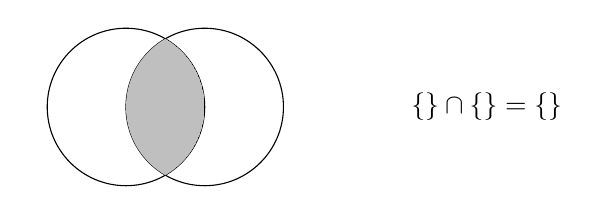
\begin{tikzpicture}[
		baseline=(current bounding box.north),
		set/.style = {
			circle,
			draw,
			minimum size = 2cm
		}
	]
	\node[set, label={180:\SM}] (M1) at (0,0) {};
	\node[set, label={  0:\SM}] (M2) at (1,0) {};
	\begin{scope}
		\clip (0,0) circle(1cm);
		\clip (1,0) circle(1cm);
		\fill[lightgray](0,0) circle(1cm);
	\end{scope}
	\node at (.5,0) {\SM};
	\node[anchor=west,align=left] at (3.5,0) {$\{\SM\} \cap \{\SM\} = \{\SM\}$};
	\end{tikzpicture}
	\label{fig:sexintersect_1}
}

\subfloat[Kombination von belebten Feminina]{
	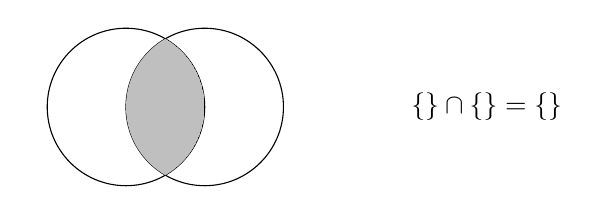
\begin{tikzpicture}[
		baseline=(current bounding box.north),
		set/.style = {
			circle,
			draw,
			minimum size = 2cm
		}
	]
	\node[set, label={180:\SF}] (F1) at (0,0) {};
	\node[set, label={  0:\SF}] (F2) at (1,0) {};
	\begin{scope}
		\clip (0,0) circle(1cm);
		\clip (1,0) circle(1cm);
		\fill[lightgray](0,0) circle(1cm);
	\end{scope}
	\node at (.5,0) {\SF};
	\node[anchor=west,align=left] at (3.5,0) {$\{\SF\} \cap \{\SF\} = \{\SF\}$};
	\end{tikzpicture}
	\label{fig:sexintersect_2}
}

\subfloat[Kombination von belebtem Maskulinum und Femininum]{
	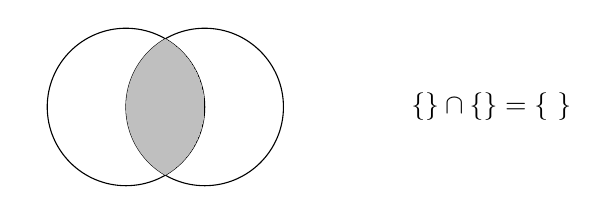
\begin{tikzpicture}[
		baseline=(current bounding box.north),
		set/.style = {
			circle,
			draw,
			minimum size = 2cm
		}
	]
	\node[set, label={180:\SM}] (M) at (0,0) {};
	\node[set, label={  0:\SF}] (F) at (1,0) {};
	\begin{scope}
		\clip (0,0) circle(1cm);
		\clip (1,0) circle(1cm);
		\fill[lightgray](0,0) circle(1cm);
	\end{scope}
	\node at (.5,0) {};
	\node[anchor=west,align=left] at (3.5,0) {$\{\SM\} \cap \{\SF\} = \{\ \}$};
	\end{tikzpicture}
	\label{fig:sexintersect_3}
}
\label{fig:sexintersect}
\caption{Kombination der Sexus-Merkmale belebter Controller}
\end{figure}

Die Menge an Belegen für den direkten Bezug zwischen Controller und Target ist
sowohl im \CAO{} als auch in der \KC{} sehr klein
(vgl.~\cref{subsubsec:perscombsgnp,subsubsec:conomctrlpers}). Ein Beispiel für
die Kombination zweier weiblicher Controller mit direktem Bezug zum Target kann
im gesammelten Belegmaterial nicht gefunden werden.%
%
	\footnote{Kursorische Suchen im \CAO{} sowie im \citetitle{rem}
	nach kombinierten belebten Feminina, die direkt durch eine adjektivisch
	flektierende Wortart modifiziert werden, waren ergebnislos.}
%
Das Diagramm in \cref{fig:sexintersect_2} ist daher eine begründete Annahme, die
sich auf Belege mit indirektem Bezug zwischen Controller und Target stützt
(siehe~\cref{subsec:beid2p2coordrefl}). Das Beispiel in \cref{ex:dietwill3}
zeigt die Kombi\-nation zweier männlicher Personen; ein Beispiel für die
Kombination einer männlichen und einer weiblichen Person wurde bereits in
\cref{ex:gendres2} gegeben.

\begin{exe}
\ex\label{ex:dietwill3}
	% \begin{xlist}
	% \ex \label{ex:dietwill3_2}
	% 	\begin{taggedline}{\parencite[\pno~83\vb, 36--37]{kc:C1}}
		\gll \textbf{Willehalm} vnd \textbf{Dietreich}. \\
			Willehalm[\Nom.\Sg.\MascM] und Dietrich[\Nom.\Sg.\MascM] \\
	\sn \gll wurden \textbf{baíde} da erſlagen. \\
			wurden beide-\Nom.\Pl.\MascM.\St{} da erschlagen \\
	% 	\end{taggedline}

	% \ex \label{ex:dietwill3_3}
	% 	\gll \textbf{Wilhalm} vnd \textbf{dietrich} \\
	% 		Willehalm[\Nom.\Sg.\MascM] und Dietrich[\Nom.\Sg.\MascM] \\
	% 	\gll Wurden \textbf{baide} do erſlagen \\
	% 		wurden beide-\Nom.\Pl.\MascM.\St{} da erschlagen \\
	% 	\begin{taggedline}{\parencites[\pno~95\vb, 12--13]{kc:K}}
		\begin{taggedline}{\parencites[\pno~83\vb, 36--37]{kc:C1}[vgl.][\pno~95\vb, 12--13]{kc:K}}
		\trans \wdef{Willehalm und Dietrich wurden beide dort erschlagen.}
		\end{taggedline}
	% \end{xlist}
\end{exe}

\textcites[576]{wechsler2009}[182]{wechslerzlatic2003} folgend lässt sich die
Situation auch für das Mittelhochdeutsche so erklären, dass zwei Typen von
Genera unterschieden werden können: einerseits Genera mit semantischen
Korrelaten wie das Maskulinum und das Femininum und andererseits Genera ohne
semantische Korrelate wie das Neutrum.

\subsubsection{Unbelebte kombinierte Controller}
\label{subsubsec:x+x_dir_inan}

Der einzige Beleg im gesammelten Material für den direkten Bezug des Targets
auf zwei unbelebte Controller ist der in \cref{ex:hofzehntbeidiu} zitierte, der
mit \lit{hof} \wdef{Hof} und \lit{zehenden} \wdef{Zehnten} zwei Maskulina
enthält. Diese werden durch pronominal verwendetes \lit{beidev} aufgenommen,
der Form nach ein Neutrum. Dasselbe Muster zeigt sich beim indirekten Bezug
zwischen Controllern und Target noch weitere vier Male im \CAO{}. Die
Frage ist, inwiefern dies Regel oder Ausnahme darstellt. In regelmäßigen Fällen
ist zu erwarten, dass zwei maskulin-unbelebte Controller ein ebenfalls
maskulines Target produzieren.

\begin{exe}
\ex\label{ex:hofzehntbeidiu}
	\gll minen \textbf{hof} \textelp{} verkaufft han mit dem
			\textbf{zehenden} \textelp{}, \textbf{beidev} vnuerſchaidenlichen
			fvͤr reht aigen \\
			meinen Hof[\Acc.\Sg.\MascI] {} verkauft habe mit dem
			Zehnt-\Dat.\Sg.\MascI{} {} beide-\Acc.\Pl.\NeutI.\St{}
			gleichermaßen für rechtmäßig Eigentum \\
	\begin{taggedline}{\parencites(Augsburg, 1283)[\pno~N~241, 195.37--39]{cao5}}
	\trans \wdef{meinen Hof verkauft habe mit dem Zehnten \textelp{}, beide
		gleichermaßen zum rechtmäßigen Eigentum}
	\end{taggedline}
\end{exe}

Die Resolutionsform von Inanimata wird \posscite{wechsler2009} Modell
zufolge durch die Schnittmenge zwischen den grammatischen Genera der Konjunkte
und deren Schnittmenge mit der Menge der formalen Korrelate der semantischen
Geschlechter ($\SM \sim \M$; $\SF \sim \F$) gebildet. Da das Neutrum die
Resolutionsform darstellt, ist es mit $\{\ \}$ definiert
\autocites[vgl.][576--578]{wechsler2009}[184--186]{wechslerzlatic2003}. Damit
ergibt sich für das Mittelhochdeutsche ein ähnliches System wie im Färöischen
oder im Isländischen
\autocites(vgl.~\cref{ex:iclgr,fig:iclgr})[225--226]{thrainsson2004}{wechsler2009}.
Anders als das Mittelhochdeutsche besitzen diese im Nom.~Pl. (Isländisch auch
im Akk.~Pl.) der starken Adjektivdeklination unterschiedliche Endungen für die
einzelnen Genera.%
%
	\footnote{Für das Färöische bzw.\ das Isländische geben
		\textcites[100--101]{thrainsson2004}[84--90]{kress1982} an:
		\fw{-ir}/\fw{-ar}/-Ø (Nom.~Pl.~M./F./N.) bzw.\ \fw{-a(r)}/\fw{-ar}/-Ø
		(Akk.~Pl.~M./F./N.). Dem gegenüber steht mhd.-obd.
		\fw{-e}/\fw{-e}/\fw{-iu} (Nom./Akk.~Pl.~M./F./N.;
		\cite[182--183]{ksw2}); siehe auch \cref{tab:faerislmhdadj}.%
	}

\begin{exe}
\needspace{3\baselineskip}
\ex \label{ex:iclgr}
	Isländisch \autocites[nach][578]{wechsler2009}[186]{wechslerzlatic2003}
	
	$G_s = \{\M, \F\}$

	\begin{tabular}[b]{@{} >{\scshape}l @{~} l l @{}}
		masc: & $\{\M\}$ & ($\gets \SM$) \\
		fem:  & $\{\F\}$ & ($\gets \SF$) \\
		neut: & $\{\ \}$  & (expletives Genus) \\
	\end{tabular}

	% \begin{tabular}[b]{
	% 	@{}
	% 	>{\scshape}l @{~\&~} >{\scshape}l @{~$=$~} >{\scshape}l
	% 	l @{~$\cap$~} l @{~$\cap~G_s =$~} l
	% 	@{}
	% }
	% 	masc & masc & masc	& $\{\M\}$ & $\{\M\}$ & $\{\M\}$ \\
	% 	fem  & fem  & fem   & $\{\F\}$ & $\{\F\}$ & $\{\F\}$ \\
	% 	neut & neut & neut  & $\{~\} $ & $\{~\} $ & $\{~\} $ \\
	% 	masc & fem  & neut  & $\{\M\}$ & $\{\F\}$ & $\{~\} $ \\
	% 	masc & neut & neut  & $\{\M\}$ & $\{~\} $ & $\{~\} $ \\
	% 	fem  & neut & neut  & $\{\F\}$ & $\{~\} $ & $\{~\} $ \\
	% \end{tabular}
\end{exe}

\begin{figure}
\centering
	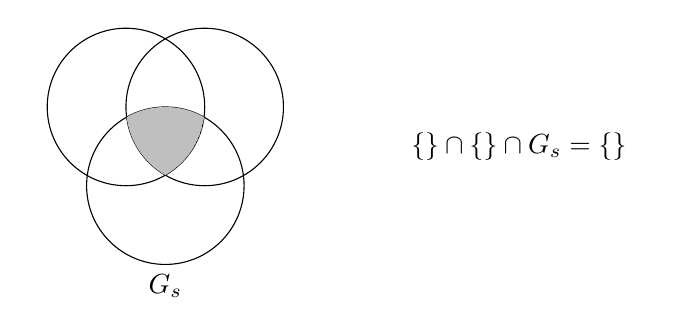
\begin{tikzpicture}[
		baseline=(current bounding box.north),
		set/.style = {
			circle,
			draw,
			minimum size = 2cm
		}
	]

	\node[set, label={180:\M}]    (M1) at (0.0,+0.5) {};
	\node[set, label={  0:\M}]    (M2) at (1.0,+0.5) {};
	\node[set, label={270:$G_s$}] (M3) at (0.5,-0.5) {};

	\begin{scope}
		\clip (0.0,+0.5) circle(1cm);
		\clip (1.0,+0.5) circle(1cm);
		\clip (0.5,-0.5) circle(1cm);
		\fill[lightgray](0.0,+0.5) circle(1cm);
	\end{scope}

	\node at (barycentric cs:M1=1,M2=1) [above]       {\M};
	\node at (barycentric cs:M1=1,M3=1) [below left]  {\M};
	\node at (barycentric cs:M2=1,M3=1) [below right] {\M};
	\node at (barycentric cs:M1=1,M2=1,M3=1) {\M};

	\node[anchor=west,align=left] at (3.5,0) {
		$\{\M\} \cap \{\M\} \cap G_s = \{\M\}$
	};
	\end{tikzpicture}
\caption%
	[Kombination unbelebter Maskulina im Isländischen]%
	{Kombination unbelebter Maskulina im Isländischen nach
	\textcites[578]{wechsler2009}[186]{wechslerzlatic2003}}
\label{fig:iclgr}
\end{figure}

% \begin{table}
% \centering
% \caption{Pluralsuffixe der starken Adjektivdeklination im Isländischen, Färöischen und Mittelhochdeutschen}
% \begin{tabular}{
% 		l
% 		c c c
% 		c
% 		c c c
% 		l
% 	}

% 	\toprule

% 	%
% 		& \mc{3}{c}{\textbf{Nom.~Pl.}}
% 		& %
% 		& \mc{3}{c}{\textbf{Akk.~Pl.}}
% 		& \mr{2}{*}[-.5ex]{\textbf{Quelle}}
% 		\\

% 	\cmidrule{2-4}
% 	\cmidrule{6-8}

% 	%
% 		& \textit{M.}
% 		& \textit{F.}
% 		& \textit{N.}
% 		& %
% 		& \textit{M.}
% 		& \textit{F.}
% 		& \textit{N.}
% 		& %
% 		\\

% 	\midrule

% 	Fär.
% 		& ir
% 		& ar
% 		& Ø
% 		& %
% 		& ar
% 		& ar
% 		& Ø
% 		& \citet[100--101]{thrainsson2004}
% 		\\

% 	\midrule

% 	Isl.
% 		& ir
% 		& ar
% 		& Ø
% 		& %
% 		& a
% 		& ar
% 		& Ø
% 		& \citet[84--90]{kress1982}
% 		\\

% 	\midrule

% 	Mhd. (obd.)
% 		& e
% 		& e
% 		& iu
% 		& %
% 		& e
% 		& e
% 		& iu
% 		& \citet[182--183]{ksw2}
% 		\\

% 	\bottomrule
% \end{tabular}
% \label{tab:fariclmhd}
% \end{table}

Aus den Regeln in \cref{ex:iclgr} ergibt sich das Resultat in \cref{fig:iclgr},
das beim Bezug von \norm{bėide} auf zwei Maskulina eintritt. In den zwei
regelmäßigen Fällen im Belegmaterial \cref{ex:m+m_inan_e} unterscheiden die
betreffenden Urkunden in der Grafie deutlich zwischen den Typen \norm{-e} und
\norm{-iu}. Der regelmäßige Fall mit \norm{-e} ist im \CAO{} zweimal
belegt und damit über\-raschender\-weise weniger häufig als die fünf Fälle mit
neutraler Kongruenz wie in \cref{ex:hofzehntbeidiu}, die sich mit dem hier
vorgestellten theoretischen Ansatz nicht erklären lassen.

\begin{exe}
\ex \label{ex:m+m_inan_e}
	\begin{xlist}
	\ex \label{ex:m+m_inan_e_1}
		\gll vn̄ ain \textbf{zehent} in der pleſwicz · vn̄ ze Belen ain
				\textbf{zehent} \textbf{die} \textbf{paid} von dē patriarch ze
				lehent ſint \\
			und ein Zehnt[\Acc.\Sg.\MascI] in der Pleschivetz {} und zu
				Wöllan ein Zehnt[\Acc.\Sg.\MascI] \Rel.\Nom.\Pl.\MascI{}
				beide[\Nom.\Pl.\MascI] von dem Patriarch zu Lehen sind \\
		\begin{taggedline}{\parencites%
			(Haimburg, Bz.~Völkermarkt, 1296)
			[\pno~2401, 487.8--9]{cao3}[vgl.][502]{caor}}
		\trans \wdef{und einen Zehnten in Plešivec und in Velenje einen
			Zehnten, die beide vom Patriarchen zum Lehen sind}
		\end{taggedline}

	\ex \label{ex:m+m_inan_e_2}
		\gll einen \textbf{Weingarten} \textelp{} Vnd einen \textbf{Chr\sscr{v}{o}tgarten}
				\textelp{} · \textbf{die} geltent \textbf{beide} ſechſthalben
				ſchillinch \textelp{} \\
			einen Weingarten[\Acc.\Sg.\MascI] {} und einen
				Gemüsegarten[\Acc.\Sg.\MascI] {} {} \Dem.\Nom.\Pl.\MascI{}
				gelten beide-\Nom.\Pl.\MascI.\St{} sechsthalben Schilling {} \\
		\begin{taggedline}{\parencites%
			(Regensburg, 1296)
			[\pno~2396, 484.28--30]{cao3}}
		\trans \wdef{einen Weingarten \textelp{} und einen Gemüsegarten
			\textelp{}, die bringen beide fünfeinhalb Schillinge \textelp{}
			ein.}
		\end{taggedline}
	\end{xlist}
\end{exe}

\subsection{Indirekter Bezug zwischen Controller und Target}
\label{subsec:beid2p2coordrefl}

Wie bereits festgestellt, sind Kontexte, in denen das Target \norm{bėide} von
einem Pronomen abhängt, wesentlich häufiger als der direkte Bezug auf zwei
nominale Controller. Dabei hat das Target nur eine indirekte Verbindung zu
seinen nominalen \q*{Erstcontrollern}. Im ausgewerteten Material sind die
Kombinationen von referenzierten Personenmerkmalen in diesem Kontext
vielfältiger als beim direkten Bezug, doch zeigen sich die gleichen Muster. Die
Untersuchung der Distanz zwischen Controller und Target (siehe dazu
\cref{sec:caotargdist,sec:kctargdist}) hat ergeben, dass die Targets in diesen
Fällen sehr häufig in Kontaktstellung (\ref{ex:pronindir_1}) und seltener in
Distanzstellung (\ref{ex:pronindir_2}) zu ihren direkten Controllern stehen;
dasselbe beobachten auch \citet[624]{ksw2}. Mitunter lässt sich die
syntaktische Domäne nicht eindeutig feststellen, da manchmal beide Lesarten --
gefloatet und nicht-gefloatet, kollektiv und distributiv -- auch in
Kontaktstellung möglich sind, insbesondere, wenn \norm{si bėide} wie in
\cref{ex:pronindir_1} das Objekt darstellt (vgl.~\cref{sec:floatquant} zu
Analysemöglichkeiten der Konstituentenstruktur).

\begin{exe}
\ex \label{ex:pronindir}
	\begin{xlist}
	\ex \label{ex:pronindir_1}
		\gll vn̄ het er ir {die ſelben} \textbf{Matta} vfgegeben lidig vn̄ lere /
			vn̄ het \textbf{ſi} \textbf{beide} von ir enphangen \\
			und hat er ihr dieselben Wiese[\Acc.\Pl.\FemI] aufgegeben ledig und
			leer {} und hat \Tpl\subI.\Acc{} beide-\Acc.\Pl.\M+\F\subI.\St{} von
			ihr empfangen \\
		\begin{taggedline}{\parencites(Freiburg i.\,Br., 1297)[\pno~2733, 105.23--24]{cao4}}
		\trans \wdef{außerdem hat er dieselben Wiesen frei und leer an sie
			ausgehändigt und hat sie beide von ihr \textins{als Lehen zurück}%
			empfangen}
		\end{taggedline}
		% \\

		% \begin{forest} shorter edges, italic leaves, nice empty nodes
		% % [CP
		% % 	[\anno{\xhead{C}}
		% % 		[und, tier=words]
		% % 	]
		% % 	[\anno{CP}
		% 	[\dots
		% 		[,phantom]
		% 		% [\anno{\xhead{C}}
		% 		% 	[het, tier=words]
		% 		% ]
		% 		[\anno{VP}
		% 			[{\anno[\pass{\Obj}]{DP\mysn{pronindir1_DP}}}
		% 				[\anno{\xhead{D}}
		% 					[ſi, tier=words]
		% 				]
		% 				[\anno{QP\mysn{pronindir1_QP}}
		% 					[\anno{\xhead{Q}}
		% 						[{%
		% 							beide \\
		% 							\smaller[2]\upshape\tabcolsep=.5ex%
		% 							\begin{tabular}[t]{@{} l l l @{}}
		% 							\ups{\GF~\Gend} & \req & $\M \lor \F$ \\
		% 							\end{tabular}%
		% 						}, tier=words]
		% 					]
		% 				]
		% 			]
		% 			[]
		% 			% [\anno{VP}
		% 			% 	[{\anno[\pass{\Oblq{\theta}}]{PP}}
		% 			% 		[\anno{\xhead{P}}
		% 			% 			[von, tier=words]
		% 			% 		]
		% 			% 		[{\anno[\pass{\Obj}]{DP}}
		% 			% 			[\anno{\xhead{D}}
		% 			% 				[ir, tier=words]
		% 			% 			]
		% 			% 		]
		% 			% 	]
		% 			% 	[\anno{\xhead{V}}
		% 			% 		[enphangen, tier=words]
		% 			% 	]
		% 			% ]
		% 		]
		% 	]
		% % ]
		% \end{forest}
		% % \hfill
		% \hspace{2em}
		% \adjustbox{valign=t}{%
		% % \smaller
		% \avm{%
		% $f:$ [
		% 	\mc{2}{c}{\dots} \\
		% 	%
		% 	\Obj	& \tikzmark{pronindir1_obj1}$g:$ [
		% 		\Pred	& $pro$ \\
		% 		\Pers	& \Third \\
		% 		\Num	& \Pl \\
		% 		\Gend	& \F \\
		% 		\Quant	& [
		% 			\Pred	& \wdef{beide} \\
		% 		] \\
		% 	]\tikzmark{pronindir1_obj2}\\
		% 	%
		% 	\mc{2}{c}{\dots}
		% ]%
		% }}
		% \begin{tikzpicture}[remember picture, overlay]
		% 	\draw [myarrow]
		% 		([yshift=.5ex]{pic cs:pronindir1_QP})
		% 		to [out=east, in=west]
		% 		([yshift=.5ex]{pic cs:pronindir1_obj1});
		% 	\draw [myarrow]
		% 		([yshift=.5ex]{pic cs:pronindir1_DP})
		% 		to [out=east, in=west]
		% 		([yshift=.5ex]{pic cs:pronindir1_obj1});
		% \end{tikzpicture}

	\ex \label{ex:pronindir_2}
		\gll die \textbf{herren} chomen wider dô. \\
			die Herren[\Nom.\Pl.\MascM] kamen wieder dahin \\
		% \gll da \textbf{ſi} voͤr der engel vant. \\
		% 	da \Tpl\subM.\Acc{} vor der Engel fand \\
		% \gll ir vart waz wol gewant. \\
		% 	ihr Reise war gut beschaffen \\
		\textelp{}
	\sn \gll \textbf{si} frævten ſich \textbf{baide} da. \\
			\Tpl\subM.\Nom{} freuten sich beide-\Nom.\Pl.\MascM.\St{} da \\
		\begin{taggedline}{\parencites[\pno~11\rb, 7--10]{kc:C1}[vgl.][\pno~11\vb, 12--15]{kc:K}[2055--2058]{schroeder1895}}
		\trans \wdef{Die Herren kamen wieder dahin
			% , wo sie der Engel zuvor gefunden hatte. Ihre Reise war gut
			% verlaufen \textins{?}.
			\textelp{}.
			Sie freuten sich da beide.}
		\end{taggedline}
		% \\

		% \begin{forest} shorter edges, italic leaves, nice empty nodes
		% [CP
		% 	[{\anno[\elem{\Top}]{DP\mysn{pronindir2_DP}}}
		% 		[\anno{\xhead{D}}
		% 			[si, tier=words]
		% 		]
		% 	]
		% 	[\anno{\xbar{C}}
		% 		[]
		% 		% [\anno{\xhead{C}}
		% 		% 	[frævten, tier=words]
		% 		% ]
		% 		[\anno{VP}
		% 			[]
		% 			% [DP
		% 			% 	[\xhead{D}
		% 			% 		[sich, tier=words]
		% 			% 	]
		% 			% ]
		% 			[\anno{VP}
		% 				[{\anno[\elem{\Top}]{QP\mysn{pronindir2_QP}}}
		% 					[\anno{\xhead{Q}}
		% 						[{%
		% 							baide \\
		% 							\smaller[2]\upshape\tabcolsep=.5ex%
		% 							\begin{tabular}[t]{@{} l l l @{}}
		% 							\ups{\GF~\Gend} & \req & $\M \lor \F$ \\
		% 							\end{tabular}%
		% 						}, tier=words]
		% 					]
		% 				]
		% 				[]
		% 				% [AdvP
		% 				% 	[\anno{\xhead{Adv}}
		% 				% 		[da, tier=words]
		% 				% 	]
		% 				% ]
		% 			]
		% 		]
		% 	]
		% ]
		% \end{forest}
		% % \hfill
		% \hspace{2em}
		% \adjustbox{valign=t}{%
		% % \smaller
		% \avm{%
		% $f:$ [
		% 	\Top	& \tikzmark{pronindir2_top1}$g:$ [
		% 		\Pred	& $pro$ \\
		% 		\Pers	& \Third \\
		% 		\Num	& \Pl \\
		% 		\Gend	& \M \\
		% 		\Sex	& \SM \\
		% 		\Quant	& [
		% 			\Pred	& \wdef{beide} \\
		% 		] \\
		% 	]\tikzmark{pronindir2_top2}\\
		% 	%
		% 	\Subj	& \tikzmark{pronindir2_subj}\\
		% 	%
		% 	\mc{2}{c}{\dots}
		% ]%
		% }}
		% \begin{tikzpicture}[remember picture, overlay]
		% 	\draw [myarrow]
		% 		([yshift=.5ex]{pic cs:pronindir2_QP})
		% 		to [out=east, in=west]
		% 		([yshift=.5ex]{pic cs:pronindir2_top1});
		% 	\draw [myarrow]
		% 		([yshift=.5ex]{pic cs:pronindir2_DP})
		% 		to [out=east, in=west]
		% 		([yshift=.5ex]{pic cs:pronindir2_top1});
		% 	\draw [rounded corners=1ex]
		% 		([yshift=.5ex]{pic cs:pronindir2_top2})
		% 		-- ++(east:1em) |-
		% 		([yshift=.5ex]{pic cs:pronindir2_subj});
		% \end{tikzpicture}
	\end{xlist}
\end{exe}

Wie in den \namecrefs{subsubsec:beid2p2snglncao}n
\labelcref{subsubsec:beid2p2snglncao,subsubsec:beid2p2snglnkc} zum indirekten
Bezug von \norm{bėide} auf einzelne Plural-Erstcontroller gezeigt, besteht in
Fällen wie in \cref{ex:pronindir}, in denen das Target indirekt von einem
einzelnen Controller abhängt, keine Variation in der Flexion zwischen
\norm{bėide} und \norm{bėidiu} bei ansonsten gleichen Personenmerkmalen. Die
Targets flektieren stattdessen extrem regelmäßig entsprechend dem Genus (\Gend)
ihres Erstcontrollers, das heißt also, nach formalen Personenmerkmalen. Daher
findet sich in \cref{ex:f+f_kindesibeidiu} die Form \lit{peidev} in Kongruenz
mit \lit{chinde} \wdef{Kinder}.

\begin{exe}
\ex \label{ex:f+f_kindesibeidiu}
	\gll ſweſter Gerdrauden vnd ſweſter Diemvden hern wernhereſ
			\textbf{chinden} \textelp{} vnd ſwenne der vorbenannten
			\textbf{chinde} einez ſtirbet \textelp{} Di weil \textbf{ſi}
			\textbf{peidev} lebent \\
		Schwester Gertraut[\Dat.\Sg.\FemF] und Schwester Diemut[\Dat.\Sg.\FemF]
			Herrn Wernhers Kinder-\Dat.\Pl.\NeutF{} {} und so=wenn der
			vorbenannten Kind-\Gen.\Pl.\NeutF{} eines stirbt {} die Weile
			\Tpl\subF.\Nom{} beide-\Nom.\Pl.\NeutF.\St{} leben \\
	\begin{taggedline}{\parencites(Engelthal, Kr.~Nürnberger Land, 1298)[\pno~2960, 240.31--38]{cao4}}
	\trans \wdef{Schwester Gertraut und Schwester Diemut, Herrn Wernhers
		Kindern \textelp{} Und wenn eines der vorgenannten Kinder stirbt
		\textelp{} Während sie beide leben}
	\end{taggedline}

	% \avm{[
	% 	\Pred			& \wdef{Kind} \\
	% 	\Case			& \Dat \\
	% 	\textbf{\Gend}	& \textbf{\N} \\
	% 	\Num			& \Pl \\
	% 	\Pers			& \Third \\
	% 	\Sex			& \SF \\
	% ]} $\to$ \avm{[
	% 	\Pred			& $pro$ \\
	% 	\Case			& \Nom \\
	% 	\textbf{\Gend}	& \textbf{\N} \\
	% 	\Num			& \Pl \\
	% 	\Pers			& \Third \\
	% 	\Sex			& \SF \\
	% 	\Quant			& [
	% 		\Pred	& \wdef{beide} \\
	% 	]
	% ]}
\end{exe}

Interessant ist diese Stelle, weil \norm{bėide} das Personalpronomen
\norm{si} \wdef{sie} modifiziert, sodass aufgrund der Wahrscheinlichkeit für
semantische Kongruenz bei pronominaler Referenz auch eine Form vom Typ
\norm{bėide} anstelle von \norm{bėidiu} möglich wäre, wie in \cref{sec:gendsex}
ausgeführt, zumal die \lit{chinde} \wdef{Kinder} im Kontext namentlich als
weiblich identifiziert werden. Dem Zusammenhang nach handelt es sich bei ihnen
nicht notwendigerweise altersmäßig um Kinder, sondern um Kinder im
verwandt\-schaft\-lichen und rechtlichen Sinn, insofern Gertraut und Diemut
auch im Jugend- oder Erwachsenen\-alter Kinder ihrer Eltern bleiben
\autocites[\pno~2960, 240.31, 35]{cao4}[vgl.~auch][\pno~2719]{cao4}[569,
619]{caor}.

Dass sich \norm{si bėidiu} direkt auf Gertraut und Diemut bezieht, ist
zumindest unter formalen Gesichtspunkten unwahrscheinlich. Die Passage lautet
im Ganzen: \lit{vnd ſwenne der vorbenanten chinde einez ſtirbet · ſo ſchol dev
vor benant gvͦlte dem andern werden di weil ez lebet · Di weil ſi peidev lebent
ſo ſchol ſi avch in peiden werden} \wdef{Und wenn eines der vorgenannten Kinder
stirbt, soll die vorgenannte Rente dem anderen zufallen, während es lebt.
Während sie beide leben, soll sie auch ihnen beiden zufallen}
\autocite[\pno~2960, 240.37--39]{cao4}.

\subsubsection{Belebte kombinierte Controller}

Aus den Tabellen \labelcref{tab:caosimprefctrl,tab:kcsimprefctrl} zur Flexion
von \norm{bėide} beim indirekten Bezug auf zwei Erstcontroller wurde deutlich,
dass nach einem Pronomen wie
\norm{wir} \wdef{wir}, \norm{si} \wdef{sie} oder \norm{di} \wdef{die
(\Rel.\Pl)} bei übereinstimmendem Geschlecht im \CAO{} stets die Form
\norm{bėide} steht, bei unterschiedlichem Geschlecht dagegen Variation zwischen
\norm{bėidiu} \cref{ex:m+f_si_beidiu} und \norm{bėide} \cref{ex:m+f_si_beide}
herrscht.

\begin{exe}
\ex \label{ex:m+f_si_beide_iu}
	\begin{xlist}
	\ex \label{ex:m+f_si_beidiu}
		\gll hern \textbf{Perhtolden} dem Meinchovær vnd ſiner \textbf{h\sscr{o}{v}ſfrowen} ver
				Magereten vnd den chinden div \textbf{ſi} \textbf{beidiv} {mit
				ein ander} habent \\
			Herrn Berthold-\Dat.\Sg.\MascM{} dem Meinchauer und seiner
				Ehefrau[\Dat.\Sg.\FemF] Frau Margarete und den Kindern die
				\Tpl\subMF.\Nom{} beide-\Nom.\Pl.\NeutMF.\St{} miteinander
				haben \\
		\begin{taggedline}{\parencites(Regensburg, 1287)[\pno~937, 292.40--41]{cao2}}
		\trans \wdef{Herrn Berthold dem Meinchauer und seiner Ehefrau, Frau 
			Margarete, und den Kindern, die sie beide miteinander haben}
		\end{taggedline}

	\ex \label{ex:m+f_si_beide}
		\gll Her \textbf{Ernſt} · vnſer burger / vnd ver \textbf{Gerdr\sscr{o}{e}vt} ſein
				hovsvrowe / da \textbf{ſi} \textbf{baide} lebten \\
			Herr Ernst[\Nom.\Sg.\MascM] {} unser Bürger {} und Frau
				Gertrud[\Nom.\Sg.\FemF] sein Ehefrau {} als \Tpl\subMF.\Nom{}
				beide-\Nom.\Pl.\M+\F\subMF.\St{} lebten \\
		\begin{taggedline}{\parencites(Wien, 1289)[\pno~1073, 374.40--41]{cao2}}
		\trans \wdef{Herr Ernst, unser Bürger, und Frau Gertrud, seine Ehefrau,
			als sie beide am Leben waren}
		\end{taggedline}
	\end{xlist}
\end{exe}

Wie bereits bei der Diskussion der \CAO{}-Belege geschildert
(siehe~\cref{subsubsec:monoflexioncao}), ist selbst bei den wenigen Fällen von
\norm{sie bėidiu} in bairischen und \norm{siu bėide} in alemannischen Urkunden
davon auszugehen, dass die Pronomen \norm{sie} und \norm{siu} als Varianten von
invariablem \norm{si} zu werten sind \autocite[vgl.][394--396]{ksw2}. In der
\KC{} gibt es zumindest einen Beleg für \norm{bėidiu} bei kombiniertem
männlichen Bezug \cref{ex:papstkoenig5}; bei unterschiedlichem Geschlecht liegt
\norm{bėidiu} in drei von insgesamt vier Fällen vor.

\begin{exe}
\ex\label{ex:papstkoenig5} % 224
	\gll Der \textbf{papſt} vnd der \textbf{chv̂nich} \\
		der Papst[\Nom.\Sg.\MascM] und der König[\Nom.\Sg.\MascM] \\
\sn \gll Si warn zegot biderb vnd frumic \\
		sie waren {zu=Gott} brav und tüchtig \\
\sn \gll Zegot ſtuͦnt allr ir geſín \\
		{zu=Gott} stand aller ihr Sinnen \\
\sn \gll Beideu ſchatz vnd gewín \\
		beide Schatz und Gewinn \\
\sn \gll Liezzen \textbf{ſi} \textbf{beideu} gelich \\
		ließen \Tpl\subM.\Nom{} beide-\Nom.\Pl.\NeutM.\St{} gleich \\
	\begin{taggedline}{\parencites[\pno~17\vb, 30--34]{kc:B1}[vgl. abweichend][6110--6113]{schroeder1895}}
	\trans \wdef{Der Papst und der König, sie waren Gott gegenüber brav und
		tüchtig. Auf Gott war all ihr Sinnen gerichtet. Sowohl Schatz als auch
		Gewinn war ihnen beiden gleich.}
	\end{taggedline}
\end{exe}

Den Analysen von \citet{wechsler2009,wechslerzlatic2003} zufolge ist in
Sprachen mit Gender Resolution im direkten Bezug auf koordinierte Nomina mit
semantischer Kongruenz zu rechnen. Bezüglich dieses syntaktischen Kontexts
wurde dies in \cref{subsec:beid2coord} anhand der wenigen verfügbaren Beispiele
bereits deutlich. Im vorliegenden Abschnitt liegt allerdings indirekter
Bezug des Targets \norm{bėide} auf zwei nominale Controller vor. Das Schema
in \cref{fig:beid2p2coordn} illustriert diesen syntaktischen Kontext.

\begin{figure}
\centering
	\begin{tikzpicture}[baseline=(1a_lb.base)]
		\node at (0,2)  (1a)    [gray]
	                            {A};
		\node           (1a_box)[draw,gray,rectangle,fit=(1a)] {};
		\node           (1a_lb) [above=.5ex of 1a_box, gray, font=\mynodefont]
	                            {Controller 1};

		\node at (0,0)  (1b)    [gray]
		                        {B};
		\node           (1b_box)[draw,gray,rectangle,fit=(1b)] {};
		\node           (1b_lb) [above=.5ex of 1b_box, gray, font=\mynodefont]
	                            {Controller 2};    

		\node at (3,1) (2)      {sie};
		\draw (2) node (2_box1) [
		                    draw,
		                    gray,
		                    minimum height=3em,
		                    minimum width=3em,
		                    xshift=-.5ex,
		                    yshift=+.5ex,
		                    rectangle
		                ] {};
		\draw (2) node (2_box2) [
		                    draw,
		                    minimum height=3em,
		                    minimum width=3em,
		                    xshift=+.5ex,
		                    yshift=-.5ex,
		                    rectangle
		                ] {};
		\node           (2_lb1) [above=.5ex of 2_box1, gray, font=\mynodefont]
		                        {Target};
		\node           (2_lb2) [below=.5ex of 2_box2, font=\mynodefont]
		                        {Controller};

		\node at (6,1)  (3)      {beide};
		\node           (3_box)  [draw,rectangle,fit=(3)] {};
		\node           (3_lb)   [above=.5ex of 3_box, font=\mynodefont]
		                        {Target};

		\draw [-latex,gray] (1a_box) to [out=east, in=west] (2_box1);
		\draw [-latex,gray] (1b_box) to [out=east, in=west] (2_box1);
		\draw [latex-]      (3_box)  to [yshift=1.5ex]      (2_box2);
	\end{tikzpicture}
\caption{\fw{Sie} als Target und Controller gleichzeitig}
\label{fig:beid2p2coordn}
\end{figure}

Das direkte Antezedens von \norm{bėide} ist ein einzelnes Pronomen, in der
Regel ein Personal- oder Relativpronomen. Insbesondere in diesem Kontext kann
Variation beobachtet werden, wie in \cref{ex:m+f_si_beide_iu} exemplarisch
dargestellt. Es ist anzunehmen, dass die beiden möglichen Kongruenzstrategien
-- formale und semantische -- miteinander konkurrieren.
\textcites[583]{wechsler2009}[194]{wechslerzlatic2003} zufolge wird in 
Sprachen, die beide Strategien anwenden, die semantische Zuweisung von Genus
zwar gewöhnlich durch formale Gender Resolution blockiert, jedoch nicht immer
vollständig, sodass die beiden Strategien in Konkurrenz zueinander stehen.

Das Pronomen \norm{si} in \cref{fig:beid2p2coordn} definiert die grammatischen
Eigenschaften in \cref{ex:beid2p2coordn_morphlex1}: Es handelt sich um ein
Personalpronomen im Nominativ Plural. Darüber hinaus referenziert dieses
Pronomen eine Gruppe von dritten Personen mit divergierenden
Geschlechtsmerkmalen. Das Pronomen \norm{si} ist selbst formal genusindifferent.

\begin{exe}
\ex \label{ex:beid2p2coordn_morphlex1}
	\begin{tabular}[t]{@{} l @{\hspace{2em}} c @{\hspace{2em}} l}
		\norm{si}
			&	D
			&	\begin{tabular}[t]{l l l}
					\ups{\Pred}				& =	& $pro$ \\
					\ups{\Prontype}			& =	& $pers$ \\
					\ups{\Concord}			& =	& ↓ \\
						\quad\downs{\Num}	& =	& \Pl \\
						\quad\downs{\Case}	& =	& \Nom \\
						\quad\downs{\Gend}	& = & Ø \\
					\ups{\Index}			& =	& ↓ \\
						\quad\downs{\Pers}	& =	& \Third \\
						\quad\downs{\Num}	& =	& \Pl \\
						\quad\downs{\Sex}	& =	& $\SM \cap \SF$ \\
				\end{tabular}
		\\
	\end{tabular}
\end{exe}

Das Target \norm{bėide} in \cref{ex:beid2p2coordn_morphlex2} kongruiert mit
seinem Controller in den formalen Merk\-malen (\Concord): Kasus (\Case), Genus
(\Gend) und Numerus (\Num). Darüber hinaus koindiziert (\Index) es seinen
Controller mit dessen Merkmalen Person (\Pers), Numerus (\Num) und Geschlecht
(\Sex). Formal wird vom Pronomen \norm{si} aber kein Genus (\Gend) festgelegt,
mit dem sein Target kongruieren könnte.

Das im ausgewerteten Material hauptsächlich beobachtete Muster entspricht der
gängigen Annahme, dass Kongruenztargets semantische Kongruenz dort zeigen, wo
der Controller für formale Kongruenzmerkmale lexikalisch nicht spezifiziert ist
\autocite[vgl.][191]{bresnanetal2016},%
%
	\footnote{\foreignblockcquote{english}[191]{bresnanetal2016}{%
		\textins*{A}greement targets \textelp{} show semantic agreement
		\emph{when the controller is lexically unspecified for the grammatical
		agreement features}}. An der zitierten Stelle ist
		\textquote{grammatical} als \q*{formal} in Bezug auf das
		\Concord-Merkmal zu verstehen.%
	}
%
Das semantische Sexusmerkmal wird also in Abwesenheit des formalen
Genusmerkmals verwendet, um Kongruenz zu ermöglichen
\cref{ex:beid2p2coordn_morphlex2}. Die Kombination von männlicher und
weiblicher Referenz wird daher am Target zu einem Neutrum aufgelöst.

\begin{exe}
\ex \label{ex:beid2p2coordn_morphlex2}
	\begin{tabular}[t]{@{} l @{\hspace{2em}} c @{\hspace{2em}} l}
		\norm{bėidiu}
			&	Q
			&	\begin{tabular}[t]{l l l}
					\ups{\Pred}				& =		& \wdef{beide} \\
					\ups{\Index}			& =		& ↓ \\
						\quad\downs{\Pers}	& =		& \Third \\
						\quad\downs{\Num}	& =		& \Pl \\
						\quad\downs{\Sex}	& =		& $\SM \cap \SF$
							\tikzmark{b2p2cml1_sex}\\
					\ups{\GF~\Concord}		& =		& ↓ \\
						\quad\downs{\Case}	& \req	& \Nom \\
						% \quad\downs{\Gend}	& \req	& \{\ \}
						% 	\tikzmark{b2p2cml1_gend}\\
						\quad\downs{\Num}	& \req	& \Pl \\
				\end{tabular}
		\\
	\end{tabular}
	\begin{tikzpicture}[remember picture, overlay]
		% \draw [-latex,	rounded corners=1ex]
		% 	([yshift=.5ex]{pic cs:b2p2cml1_sex})
		% 	-- ++(east:1em) |-
		% 	([yshift=1ex]{pic cs:b2p2cml1_gend});
		% \draw [-latex]
		% 	([yshift=0ex]{pic cs:b2p2cml1_gend})
		% 	-- ++(east:5em) node[anchor=west] {\N\ (\norm{-iu})};
		\draw [-latex]
			([yshift=1ex]{pic cs:b2p2cml1_sex})
			-- ++(east:3em) node[anchor=west] {\N\ (\norm{-iu})};
	\end{tikzpicture}
\end{exe}

Um die trotz allem vorkommende Form \norm{bėide} zu erklären, wäre denkbar,
dass die Information des Sexusmerkmals formal interpretiert wird
\cref{ex:beid2p2coordn_morphlex4}: Ein Flexiv, das Maskulina und Feminina
gleichermaßen bezeichnet, ist mit \norm{-e} vorhanden. Da das Pronomen kein
Genusmerkmal definiert, läge auch damit keine Verletzung von
morphosyntaktischen Beschränkungen vor.

\begin{exe}
\ex \label{ex:beid2p2coordn_morphlex4}
	\begin{tabular}[t]{@{} l @{\hspace{2em}} c @{\hspace{2em}} l}
		\norm{bėide}
			&	Q
			&	\begin{tabular}[t]{l l l}
					\ups{\Pred}				& =		& \wdef{beide} \\
					\ups{\Index}			& =		& ↓ \\
						\quad\downs{\Pers}	& =		& \Third \\
						\quad\downs{\Num}	& =		& \Pl \\
						\quad\downs{\Sex}	& =		& $\SM \cap \SF$
							\tikzmark{b2p2cml2_sex}\\
					\ups{\GF~\Concord}		& =		& ↓ \\
						\quad\downs{\Case}	& \req	& \Nom \\
						\quad\downs{\Gend}	& \req	& $\M \lor \F$
							\tikzmark{b2p2cml2_gend}\\
						\quad\downs{\Num}	& \req	& \Pl \\
				\end{tabular}
		\\
	\end{tabular}
	\begin{tikzpicture}[remember picture, overlay]
		\draw [-latex, rounded corners=1ex]
			([yshift=.5ex]{pic cs:b2p2cml2_sex})
			-- ++(east:1em) |-
			% node [near start, right] {\mynodefont Reinterpretation}
			([yshift=1ex]{pic cs:b2p2cml2_gend});
		\draw [-latex]
			([yshift=0ex]{pic cs:b2p2cml2_gend})
			-- ++(east:3em) node[anchor=west] {\M+\F\ (\norm{-e})};
	\end{tikzpicture}
\end{exe}

Insofern angenommen werden kann, dass \norm{si bėide} bei Kontaktstellung eine
Phrase bildet, unterscheiden sich die betreffenden Schreiberinnen und Schreiber
der ausgewerteten Quellen vermutlich also in der Präferenz der anzuwendenden
Regel, das heißt, ob sie in Zweifelsfällen semantische Kongruenz oder formale
Kongruenz basierend auf semantischen Informationen anwenden. Im Belegmaterial
jedenfalls wird die \norm{iu}-Form stark bevorzugt, sehr regelmäßig sogar in
dem anderen syntaktischen Kontext mit eindeutiger Distanzstellung von
\wdef{beide}, wie in \cref{ex:m+f_si_beidiu_float} illustriert
(vgl.~auch \cref{tab:caoanadist,tab:kcanadist} zur Wortdistanz zwischen
\norm{bėide} und einem pronominalen Controller).

\begin{exe}
\ex \label{ex:m+f_si_beidiu_float}
	\gll vnd ſol {der ſelbe} \textbf{vlrich} / oder fraw \textbf{Margret} \textelp{}
			\textbf{ſi} leben \textbf{peidev} ſamte / oder ir æintwederez \\
		und soll derselbe Ulrich[\Nom.\Sg.\MascM] {} oder Frau
			Margarete[\Nom.\Sg.\FemF] {} \Tpl\subMF.\Nom{} leben
			beide-\Nom.\Pl.\NeutMF.\St{} zusammen {} oder ihr
			entweder-\Nom.\Sg.\NeutMF.\St{} \\
	\begin{taggedline}{\parencites(Brixen, 1298)[\pno~3141~A, 352.3--9]{cao4}}
	\trans \wdef{Außerdem soll derselbe Ulrich oder Frau Margarete \textelp{}
		wenn sie beide zusammen am leben sind oder einer von ihnen}
	\end{taggedline}
\end{exe}

Das Target \norm{bėidiu} in \cref{ex:m+f_si_beidiu_float} befindet sich
ungeachtet der semantischen Zusammengehörigkeit in diesem Fall nicht in
derselben NP wie sein Controller \lit{vlrich / oder fraw Margret} \wdef{Ulrich
oder Frau Margarete}, daher spielt formale Kongruenz in diesem Kontext kaum
eine Rolle. Belege für gefloatetes \norm{bėide} in Bezug auf
gemischtgeschlechtliche Controller sind nur vereinzelt vorhanden, stattdessen
überwiegt semantische Kongruenz, inklusive der dabei operierenden Gender
Resolution.

Bezüglich der Kongruenzhierarchie (vgl.~\cref{sec:kongrhier}) stellt sich die
Frage, in welcher Kongruenzdomäne gefloatete Quantoren einzuordnen sind. Im
Modell von \textcites{corbett1979}[84]{wechslerzlatic2003} tauchen sie als
solche nicht auf. Zumindest beim kombinierten belebten Bezug ist regelmäßig die
neutrale statt der maskulin-femininen Form zu beobachten, wahrscheinlich
aufgrund von Gender Resolution, was widerum auf Koindizierung hinweist. Geht
man mit \citet{spector2009} aufgrund semantischer Differenzen (die auch
\cite{pittner1995} beobachtet) davon aus, dass Kontakt- und Distanzstellung von
Quantoren nicht nur semantisch, sondern auch funktional zu unterscheiden sind
(vgl.~dazu in \cref{phsec:hebrqf}), müsste ein Floating Quantifier mit
Subjektsbezug in dem Schema in \cref{fig:theoagrdist} neben dem primären
Prädikat (zum Beispiel prädikative Adjektive) anzusiedeln sein, da auch dieses
in einem anderen Satzteil desselben Teilsatzes steht und semantisch ein
Attribut des Subjekts darstellt. Nach der gröberen Einteilung von
\citet[216]{corbett1979} sollte es neben dem Relativpronomen stehen, da es
außerhalb des Satzteils seines Controllers steht, doch auf denselben Satz
beschränkt bleibt, in jedem Fall jedoch vor dem Personalpronomen, dessen Domäne
über den Satz hinausgeht.%
% %
% 	\footnote{\foreignblockcquote{english}[216]{corbett1979}{\textins*{T}he
% 		agreement of the relative pronoun goes beyond the clause but is
% 		restricted to the sentence, while the personal pronoun is not
% 		restricted to the sentence of the item controlling agreement}.%
% 	}

\subsubsection{Unbelebte kombinierte Controller}

Beim indirekten Bezug auf kombinierte unbelebte Controller steht ebenfalls nur
Belegmaterial aus dem \CAO{} zur Verfügung. Wie bei der Auswertung zur
Kongruenz von \norm{bėide} im indirekten Bezug auf kombinierte nominale
Controller in \cref{subsubsec:beid2p2coordncao} beobachtet, ist der häufigste
Fall in unbelebten Kontexten eine Form des Typs \norm{bėidiu} unabhängig vom
Genus der Controller, wobei die Kombination zweier unbelebter Feminina nicht
belegt ist. Daneben stehen die zwei Belege in \cref{ex:m+m_inan_e2}, die die
maskulin-feminine Form \norm{bėide} in Einklang mit maskulinen Controllern
enthalten. Auch die zahlreichen Belege für \norm{bėidiu} mit indirektem Bezug
auf zwei Neutra \cref{ex:insigel} sind unauffällig. Gegenbelege mit
\norm{bėide}, die einer Erklärung bedürften, liegen keine vor.

\begin{exe}
\ex \label{ex:m+m_inan_e2}
	\begin{xlist}
	\ex \label{ex:m+m_inan_e2_1}
		\gll vn̄ ain \textbf{zehent} in der pleſwicz · vn̄ ze Belen ain
				\textbf{zehent} \textbf{die} \textbf{paid} von dē patriarch ze
				lehent ſint \\
			und ein Zehnt[\Acc.\Sg.\MascI] in der Pleschivetz {} und zu
				Wöllan ein Zehnt[\Acc.\Sg.\MascI] \Rel.\Nom.\Pl.\MascI{}
				beide[\Nom.\Pl.\MascI] von dem Patriarch zu Lehen sind \\
		\begin{taggedline}{\parencites%
			(Haimburg, Bz.~Völkermarkt, 1296)
			[\pno~2401, 487.8--9]{cao3}[vgl.][502]{caor}}
		\trans \wdef{und einen Zehnten in Plešivec und in Velenje einen
			Zehnten, die beide vom Patriarchen zum Lehen sind}
		\end{taggedline}
		% III.2401.487.10 vnd haben in den egenanten Tuͦren
		% III.2401.487.11 halben mit allev dew vn̄ dar ze gehoͤrt
		% [...]
		% III.2401.487.16 Daz ſuͦllen ſi haben · auf vns vn̄
		% III.2401.487.17 auf vnſern triwen · vn̄ auf alle deu vn̄ wir haben

		% \begin{forest} shorter edges, italic leaves, nice empty nodes
		% [CP
		% 	[{\anno[\elem{\Top}]{DP\mysn{mmiaiu1_DP}}}
		% 		[\anno{\xhead{D}}
		% 			[{%
		% 				die \\
		% 				\smaller[2]\upshape\tabcolsep=.5ex%
		% 				\begin{tabular}[t]{@{} l c l @{}}
		% 				\downs{\Gend}	& = & $\M \cap \M \cap G_s$ \\
		% 				% 				& $\Rightarrow $ & \M \\
		% 				\end{tabular}%
		% 			}, tier=words]
		% 		]
		% 	]
		% 	[\anno{VP}
		% 		[{\anno[\elem{\Top}]{QP\mysn{mmiaiu1_QP}}}
		% 			[\anno{\xhead{Q}}
		% 				[{%
		% 					paid \\
		% 					\smaller[2]\upshape\tabcolsep=.5ex%
		% 					\begin{tabular}[t]{@{} l l l @{}}
		% 					\ups{\GF~\Gend} & \req & $\M \lor \F$ \\
		% 					\end{tabular}%
		% 				}, tier=words]
		% 			]
		% 		]
		% 		[]
		% 	]
		% ]
		% \end{forest}
		% \hfill
		% % \hspace{2em}
		% \adjustbox{valign=t}{%
		% % \smaller
		% \avm{%
		% $f:$ [
		% 	\Top	& \tikzmark{mmiaiu1_top1}$g:$ [
		% 		\Prontype & $rel$ \\
		% 		\Pred	& $pro$ \\
		% 		\Pers	& \Third \\
		% 		\Num	& \Pl \\
		% 		\Gend	& \M \\
		% 		\Case	& \Nom \\
		% 		\Quant		& [
		% 			\Pred	& \wdef{beide} \\
		% 		] \\
		% 	]\tikzmark{mmiaiu1_top2}\\
		% 	%
		% 	\Subj	& \tikzmark{mmiaiu1_subj}\\
		% 	%
		% 	\mc{2}{c}{\dots}
		% ]%
		% }}
		% \begin{tikzpicture}[remember picture, overlay]
		% 	\draw [myarrow]
		% 		([yshift=.5ex]{pic cs:mmiaiu1_QP})
		% 		to [out=east, in=west]
		% 		([yshift=.5ex]{pic cs:mmiaiu1_top1});
		% 	\draw [myarrow]
		% 		([yshift=.5ex]{pic cs:mmiaiu1_DP})
		% 		to [out=east, in=west]
		% 		([yshift=.5ex]{pic cs:mmiaiu1_top1});
		% 	\draw [rounded corners=1ex]
		% 		([yshift=.5ex]{pic cs:mmiaiu1_top2})
		% 		-- ++(east:1em) |-
		% 		([yshift=.5ex]{pic cs:mmiaiu1_subj});
		% \end{tikzpicture}

	\ex \label{ex:m+m_inan_e2_2}
		\gll einen \textbf{Weingarten} \textelp{} Vnd einen \textbf{Chr\sscr{v}{o}tgarten}
				\textelp{} · \textbf{die} geltent \textbf{beide} ſechſthalben
				ſchillinch \textelp{} \\
			einen Weingarten[\Acc.\Sg.\MascI] {} und einen
				Gemüsegarten[\Acc.\Sg.\MascI] {} {} \Rel.\Nom.\Pl.\MascI{}
				gelten beide-\Nom.\Pl.\MascI.\St{} sechsthalben Schilling {} \\
		\begin{taggedline}{\parencites%
			(Regensburg, 1296)%
			[\pno~2396, 484.28--30]{cao3}}
		\trans \wdef{einen Weingarten \textelp{} und einen Gemüsegarten
			\textelp{}, die beide fünfeinhalb Schillinge \textelp{}
			einbringen.}
		\end{taggedline}
		% III.2396.484.30 Vnd han div ſel-
		% III.2396.484.31 ben vor genanten gvͦt elliv driv zelehen enpfangen

		% \begin{forest} shorter edges, italic leaves, nice empty nodes
		% [CP
		% 	[{\anno[\elem{\Top}]{DP\mysn{mmiaiu2_DP}}}
		% 		[\anno{\xhead{D}}
		% 			[{%
		% 				die \\
		% 				\smaller[2]\upshape\tabcolsep=.5ex%
		% 				\begin{tabular}[t]{@{} l c l @{}}
		% 				\downs{\Gend}	& = & $\M \cap \M \cap G_s$ \\
		% 				% 				& $\Rightarrow $ & \M \\
		% 				\end{tabular}%
		% 			}, tier=words]
		% 		]
		% 	]
		% 	[\anno{\xbar{C}}
		% 		[]
		% 		[\anno{VP}
		% 			[{\anno[\elem{\Top}]{QP\mysn{mmiaiu2_QP}}}
		% 				[\anno{\xhead{Q}}
		% 					[{%
		% 						beide \\
		% 						\smaller[2]\upshape\tabcolsep=.5ex%
		% 						\begin{tabular}[t]{@{} l l l @{}}
		% 						\ups{\GF~\Gend} & \req & $\M \lor \F$ \\
		% 						\end{tabular}%
		% 					}, tier=words]
		% 				]
		% 			]
		% 			[]
		% 		]
		% 	]
		% ]
		% \end{forest}
		% \hfill
		% % \hspace{2em}
		% \adjustbox{valign=t}{%
		% % \smaller
		% \avm{%
		% $f:$ [
		% 	\Top	& \tikzmark{mmiaiu2_top1}$g:$ [
		% 		\Prontype & $dem$ \\
		% 		\Pred	& $pro$ \\
		% 		\Pers	& \Third \\
		% 		\Num	& \Pl \\
		% 		\Gend	& \M \\
		% 		\Case	& \Nom \\
		% 		\Quant		& [
		% 			\Pred	& \wdef{beide} \\
		% 		] \\
		% 	]\tikzmark{mmiaiu2_top2}\\
		% 	%
		% 	\Subj	& \tikzmark{mmiaiu2_subj}\\
		% 	%
		% 	\mc{2}{c}{\dots}
		% ]%
		% }}
		% \begin{tikzpicture}[remember picture, overlay]
		% 	\draw [myarrow]
		% 		([yshift=.5ex]{pic cs:mmiaiu2_QP})
		% 		to [out=east, in=west]
		% 		([yshift=.5ex]{pic cs:mmiaiu2_top1});
		% 	\draw [myarrow]
		% 		([yshift=.5ex]{pic cs:mmiaiu2_DP})
		% 		to [out=east, in=west]
		% 		([yshift=.5ex]{pic cs:mmiaiu2_top1});
		% 	\draw [rounded corners=1ex]
		% 		([yshift=.5ex]{pic cs:mmiaiu2_top2})
		% 		-- ++(east:1em) |-
		% 		([yshift=.5ex]{pic cs:mmiaiu2_subj});
		% \end{tikzpicture}
	\end{xlist}
\end{exe}

Wie aussagekräftig sind die Belege in \cref{ex:m+m_inan_e2} angesichts des
Umstands, dass der erwartete Regelfall zahlenmäßig die Ausnahme darstellt? Die
Urkunde zu \cref{ex:m+m_inan_e2_1} enthält neben \lit{mit allev dew} \wdef{mit
all dem} und \lit{auf alle deu} \wdef{auf alle die} \autocite[\pno~2401,
487.11, 17]{cao3} als Rest des Instrumentals \autocite[vgl.][618]{ksw2} nur
\norm{die} als Relativpronomen, dafür aber stets in formalem Einklang mit
seinem Controller. Anzumerken ist, dass das Relativpronomen und
\norm{bėide} in unterschiedlichen Phrasen stehen, also trotz
oberflächlicher Kontaktstellung in der C-Struktur Distanzstellung vorliegt. Da
das Relativpronomen in \cref{ex:dibeidecstruct} die Subjektsposition einnimmt
(hier die DP-Schwester von \xbar{C}) und das finite Verb im Relativsatz in der
rechten Satzklammer steht, bleibt die linke Satzklammer (\xhead{C}) leer. In
der linearen Abfolge der Wortformen steht daher \norm{bėide} direkt hinter
\norm{die}, auch wenn \norm{die} und \norm{bėide} zusammen keine Phrase bilden.

% \begin{figure}
\begin{exe}
\ex \label{ex:dibeidecstruct}
	\begin{forest} shorter edges, align text,
	[CP
		[DP
			[\xhead{D}
				[\textit{die}]
			]
		]
		[\xbar{C}
			[\xhead{C}
				[Ø]
			]
			[VP
				[QP
					[\xhead{Q}
						[\textit{beide}]
					]
				]
				[\xbar{V}
					[\dots]
				]
			]
		]
	]
	\end{forest}
\end{exe}
% \end{figure}

Die in \cref{ex:m+m_inan_e2_2} zitierte Urkunde unterscheidet zumindest beim
definiten Artikel regelmäßig zwischen \norm{die} und \norm{diu}. In beiden
Urkunden spricht nichts ausdrücklich gegen die Annahme, dass \norm{die} die maskulin-feminine Form des Relativpronomens darstellt. Das
von diesem Pronomen abhängige Target \norm{bėid(e)} kann problemlos mit dem
Genusmerkmal des jeweiligen pronominalen Controllers kongruieren, da sich
dieser auf zwei Maskulina bezieht.

Wie bei den Belegen mit direktem Bezug kann das Auftreten von neutralem
\norm{bėidiu} bei verschiedenem Geschlecht der Erstcontroller mit einer
Mengenoperation analog zu der in \cref{fig:iclgr} erklärt werden; verbildlicht
wird dies in \cref{fig:iclgr2}. Maskulin und Feminin haben zwar jeweils eine
Schnittmenge mit der Menge der semantisch gekoppelten Genera ($G_s$),
allerdings nicht miteinander. In \cref{ex:iclgr2_1} resultiert daher eine leere
Menge $\{\ \}$ die dem Neutrum als Resolutionsgenus entspricht. In den anderen
beiden Fällen mit Neutrum \crefrange{ex:iclgr2_2}{ex:iclgr2_3} kommt es nur
jeweils beim Maskulinum und beim Femininum zu einer Schnittmenge mit $G_s$,
aber nirgends sonst, sodass auch dort nur das Neutrum als Lösung bleibt.

\begin{exe}
\ex \label{ex:iclgr2}
\begin{xlist}
	\ex \label{ex:iclgr2_1}
		\gll vnd verzeih mich / \textelp{}  dez \textbf{Cehenten} vnd der \textbf{h\sscr{u}{o}b} 
				/ \textbf{dev} \textbf{paidev} {vor benemt} ſint \\
			und verzichte mich {} {} des Zehnten[\Gen.\Sg.\MascI] und der
				Hube[\Gen.\Sg.\FemI] {} \Rel.\Nom.\Pl.\NeutI{}
				beide-\Nom.\Pl.\NeutI.\St{} vorgenannt sind \\
			\begin{taggedline}{\parencites(Regensburg, 1299)[\pno~3261, 424.38--39]{cao4}}
			\trans \wdef{und verzichte \textelp{} auf den Zehnten und die Hube,
				die beide vorgenannt sind}
			\end{taggedline}

	\ex \label{ex:iclgr2_2}
		\gll einen \textbf{Hof} / vnd ein \textbf{Lehen} - da pei / \textbf{vnd} ſind
				\textbf{paidev} æigen \\
			einen Hof[\Acc.\Sg.\MascI] {} und ein Lehen[\Acc.\Sg.\NeutI] {} da
				bei {} \Rel{} sein[\Tpl\subM.\Ind.\Prs]
				beide-\Nom.\Pl.\NeutI.\St{} Eigentum \\
			\begin{taggedline}{\parencites(Steyr, 1294)[\pno~1923, 194.36--37]{cao3}}
			\trans \wdef{einen Hof und ein Lehen in der Nähe, die beide
				Eigentum sind}
			\end{taggedline}

	\ex \label{ex:iclgr2_3}
		\gll daz ich auz minem \textbf{hauz} vnd auz miner \textbf{hofſtat}
				\textbf{div} \textbf{bediv} min recht eigen ſint \textelp{} \\
			dass ich aus meinem Haus[\Dat.\Sg.\NeutI] und aus meiner
				Grundstück[\Dat.\Sg.\FemI] \Rel.\Nom.\Pl.\NeutI{}
				beide-\Nom.\Pl.\NeutI.\St{} mein rehtmäßig Eigentum sind {} \\
			\begin{taggedline}{\parencites(Ulm und Kl.~Raitenhaslach, Kr.~Altötting, 1282)[\pno~1282, 526.37--38]{cao2}}
			\trans \wdef{dass ich aus meinem Haus und aus meinem Grundstück, 
				die beide mein rechtmäßiges Eigentum sind \textelp{}}
			\end{taggedline}
	\end{xlist}
\end{exe}

\begin{figure}
\centering
\subfloat[Kombination von unbelebtem Maskulinum und Femininum]{
	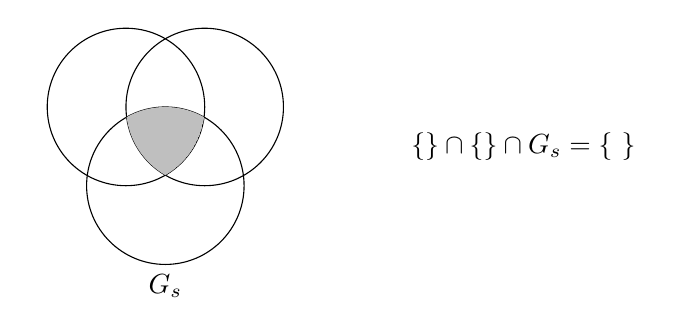
\begin{tikzpicture}[
		baseline=(current bounding box.north),
			set/.style = {
				circle,
				draw,
				minimum size = 2cm
			}
		]
		\node[set, label={180:\M}]    (M)  at (0.0,+0.5) {};
		\node[set, label={  0:\F}]    (F)  at (1.0,+0.5) {};
		\node[set, label={270:$G_s$}] (MF) at (0.5,-0.5) {};
		\begin{scope}
			\clip (0.0,+0.5) circle(1cm);
			\clip (1.0,+0.5) circle(1cm);
			\clip (0.5,-0.5) circle(1cm);
			\fill[lightgray](0.0,+0.5) circle(1cm);
		\end{scope}
		\node at (barycentric cs:M=1,MF=1) [below left]  {\M};
		\node at (barycentric cs:F=1,MF=1) [below right] {\F};
		\node at (barycentric cs:M=1,F=1,MF=1) {};
		\node[anchor=west,align=left] at (3.5,0) {
			$\{\M\} \cap \{\F\} \cap G_s = \{\ \}$
		};
	\end{tikzpicture}
}

\subfloat[Kombination von unbelebtem Maskulinum und Neutrum]{
		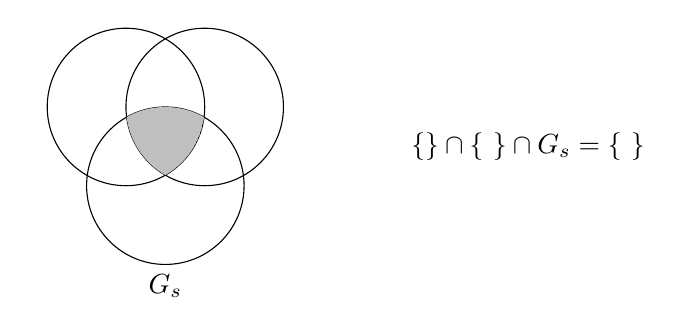
\begin{tikzpicture}[
			baseline=(current bounding box.north),
			set/.style = {
				circle,
				draw,
				minimum size = 2cm
			}
		]
		\node[set, label={180:\M}]    (M)  at (0.0,+0.5) {};
		\node[set, label={  0:}]      (N)  at (1.0,+0.5) {};
		\node[set, label={270:$G_s$}] (MF) at (0.5,-0.5) {};
		\begin{scope}
			\clip (0.0,+0.5) circle(1cm);
			\clip (1.0,+0.5) circle(1cm);
			\clip (0.5,-0.5) circle(1cm);
			\fill[lightgray](0.0,+0.5) circle(1cm);
		\end{scope}
		\node at (barycentric cs:M=1,MF=1) [below left] {\M};
		\node at (barycentric cs:M=1,N=1,MF=1) {};
		\node[anchor=west,align=left] at (3.5,0) {
			$\{\M\} \cap \{\ \} \cap G_s = \{\ \}$
		};
	\end{tikzpicture}
}

\subfloat[Kombination von unbelebtem Femininum und Neutrum]{
	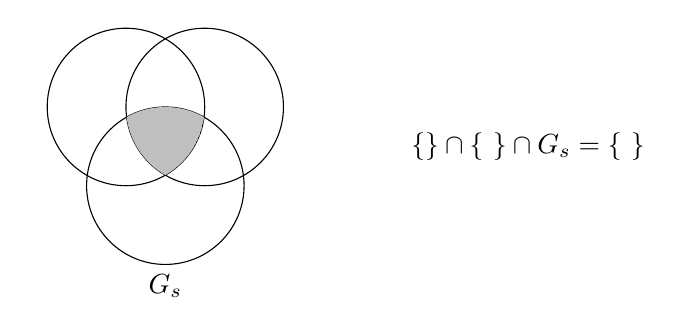
\begin{tikzpicture}[
			baseline=(current bounding box.north),
			set/.style = {
				circle,
				draw,
				minimum size = 2cm
			}
		]
		\node[set, label={180:\F}]    (F)  at (0.0,+0.5) {};
		\node[set, label={  0:}]      (N)  at (1.0,+0.5) {};
		\node[set, label={270:$G_s$}] (MF) at (0.5,-0.5) {};
		\begin{scope}
			\clip (0.0,+0.5) circle(1cm);
			\clip (1.0,+0.5) circle(1cm);
			\clip (0.5,-0.5) circle(1cm);
			\fill[lightgray](0.0,+0.5) circle(1cm);
		\end{scope}
		\node at (barycentric cs:F=1,MF=1) [below left] {\F};
		\node at (barycentric cs:F=1,N=1,MF=1) {};
		\node[anchor=west,align=left] at (3.5,0) {
			$\{\F\} \cap \{\ \} \cap G_s = \{\ \}$
		};
	\end{tikzpicture}
}
\caption{Kombination verschiedener Genusmerkmale unbelebter Controller}
\label{fig:iclgr2}
\end{figure}

\subsection{Neutrum bei maskulinem und femininem Bezug}
\label{subsec:m+m_anim_beidiu}

Neben regelmäßigen Fällen, in denen die Kombination zweier Maskulina die Form
\norm{bėide} ergibt%
% ($\{\SM\} \cap \{\SM\} \Rightarrow \{\M\}$ sowie $\{\M\}
% \cap \{\M\} \cap G_s \Rightarrow \{\M\}$)
, zeigten sich sowohl mit Bezug auf belebte als auch auf unbelebte maskuline
(Erst-)Controller mehrere Vorkommen von neutralem \norm{bėidiu}. Diese
verteilen sich auf alle untersuchten Kontexte, wie beispielhaft in
\cref{ex:m+m_beidiu} gezeigt, mit Ausnahme der Abhängigkeit von pronominalen
Controllern mit belebter Referenz.

\begin{exe}
\ex \label{ex:m+m_beidiu}
	\begin{xlist}
	\ex \label{ex:m+m_beidiu_1}
		\gll Die \textbf{rihtær} ſprachen \textbf{beideu} {dar zuͦ} \\
			die Richter[\Nom.\Pl.\MascM] sprachen beide-\Nom.\Pl.\NeutM.\St{}
			dazu \\
		\begin{taggedline}{\parencites[\pno~28\ra, 8]{kc:B1}[vgl.~abweichend][10090]{schroeder1895}} % 1140 mit Parallelstelle in H
		\trans \wdef{Die Richter äußerten sich beide dazu}
		\end{taggedline}

	% \ex \label{ex:m+m_beidiu_2}
	% 	\gll Die \textbf{herren} baten ir ſa \\
	% 		Die Herren[\Nom.\Pl.\MascM] baten ihr alsbald \\
	% 	\gll \textbf{Beideu} beſvnder \\
	% 		beide-\Nom.\Pl.\NeutM.\St{} einzeln \\
	% 	\begin{taggedline}{\parencites[\pno~31\va, 48--49]{kc:B1}[vgl.][11385--11386]{schroeder1895}} % 1112x
	% 	\trans \wdef{Die Herren hielten alsbald jeweils beide um ihre Hand an.}
	% 	\end{taggedline}

	\ex \label{ex:m+m_beidiu_3}
		\gll Diſ dingeſ gezuga ſint · \textbf{R\sscr{u}{o}d} · von der palma
				min Oͤhen · \textbf{\sscr{v}{o}lrich} von Grvͤnenberch min Oͤhen
				\textbf{bedu} Jungherren % \\
				% · hug von waltherſwile ·
				\textelp{} \\
			Dies Verhandlung-\Gen.\Sg.\NeutI{} Zeugen sind {}
				\lit{Ruͦd}[\Nom.\Sg.\MascM] {} von der Palme mein Oheim {}
				Ulrich[\Nom.\Sg.\MascM] von Grünenberg mein Oheim
				beide-\Nom.\Pl.\NeutM.\St{} Jungherren[\Nom.\Pl.\MascM] % \\
				% {} Hug von Walterswil {}
				{} \\
		\begin{taggedline}{\parencites(Kl.~St.~Urban, Kt.~Luzern, 1298)[\pno~2915, 213.33--35]{cao4}}
		\trans \wdef{Zeugen dieser Verhandlung sind: \lit{Ruͦd} von der Palme,
			mein Onkel, Ulrich von Grünenberg, mein Onkel -- beide Junker --
			% Hug von Walterswil, 
			\textelp{}}
		\end{taggedline}

	% \ex \label{ex:m+m_beidiu_4}
	% 	\gll \textbf{Karle} an daz gerichte ſaz \\
	% 	    Karl[\Nom.\Sg.\MascM] an das Gericht saß \\
	% 	\gll Der \textbf{babſt} klegt \textbf{ím} daz \\
	% 		der Papst[\Nom.\Sg.\MascM] klagte \Tsg.\MascM.\Dat{} dass \\
	% 	\gll Der wideme vnd der zehende gar \\
	% 		der Stiftungen und der Zehnten gar \\
	% 	\gll Waͤren \textbf{baidú} worden bar \\
	% 		wären beide-\Nom.\Pl.\NeutM.\St{} geworden bloß \\
	% 	\gll Von ſínen vorvarn \\
	% 		von seinen Vorfahren \\
	% 	\begin{taggedline}{\parencites[\pno~85\vb, 21--25]{kc:K}[vgl. abweichend][14382--14386]{schroeder1895}}
	% 	\trans \wdef{Karl (der Große) saß zu Gericht. Der Papst klagte ihm, dass
	% 		beide durch seine Vorgänger an Stiftungen und gar an Zehnten ledig
	% 		geworden wären.}
	% 	\end{taggedline}

	\ex \label{ex:m+m_beidiu_5}
		\gll vnſerne \textbf{zehenden} zeandeluingen vnde
				ainen \textbf{Garten} indem ſelben dorfe \textelp{}
				\textbf{div} wier \textbf{baidiv} fvr reht aigen her
				haigen~\textins{sic} braht \\
			unseren Zehnt-\Acc.\Sg.\MascI{} zu=Andelfingen und einen
				Garten-\Acc.\Sg.\MascI{} in.dem selben Dorf {}
				\Rel.\Acc.\Pl.\NeutI{} wir beide-\Acc.\Pl.\NeutI.\St{} für
				rehtmäßig Eigentum her haben gebracht \\
		\begin{taggedline}{\parencites(Kl.~Heiligkreuztal, Kr.~Biberach, 1290)[\pno~1201~AB, 472.10--14]{cao2}}
		\trans \wdef{unseren Zehnten in Andelfingen und einen Garten in
			demselben Dorf \textelp{}, die wir beide zum rechtmäßigen Eigentum
			\textins{dar}gebracht haben}
		\end{taggedline}
	\end{xlist}
\end{exe}

Der Beleg in \cref{ex:m+m_beidiu_1} enthält ein \norm{bėidiu}-Target, das sich
unmittelbar auf das Plural-Maskulinum \lit{rihtær} \wdef{Richter} bezieht, das
seinerseits männlich denotiert ist.
% -- gemeint sind die wortführenden Rabbiner, mit denen Papst Silvester in
% dieser Episode der \KC{} debattiert.
Bei \cref{ex:m+m_beidiu_3} bezieht sich \lit{bedu} entweder direkt auf die
beiden Herren \lit{Ruͦd}\textins{\norm{iger}/\norm{olf}?} und \lit{vͦlrich}
oder auf \lit{Jungherren} \wdef{Junker}. In jedem Fall ist die Kongruenzform
von \norm{bėide} anomal. Zuletzt bezieht sich die neutrale Form \lit{baidiv} in
\cref{ex:m+m_beidiu_5} dem Kontext nach am ehesten auf
\lit{zehenden} \wdef{Zehnten} und \lit{Garten} \wdef{Garten}. Da es sich bei
den Ausstellern der Urkunde um die drei Brüder \lit{wezel vn̄ hainrich wezel
vnde Cvͦnrat de}\textins*{\norm{n}}\lit{ Bodemer} \autocite[\pno~1201~AB,
472.6--7]{cao2} handelt, wird sich \lit{baidiv} nicht auf \lit{wier} beziehen.
Vielmehr wurde die Stelle so interpretiert, dass der Zehnt und der Garten
gemeinsam im Rahmen der Verkaufsverhandlung als rechtmäßiges Eigentum
dargebracht wurden.

Das theoretische Modell von \citet{wechsler2009} und \citet{wechslerzlatic2003}
vermag diese Ausnahmen nicht zu erklären. Die \cref{tab:m+m_beidiu} zeigt die
Verteilung der Formen mit Bezug auf maskulin-männliche und maskulin-unbelebte
Controller auf die unterschiedlichen belegten syntaktischen Kontexte.
Hervorzuheben ist, dass insgesamt lediglich neun Belege in der gesamten
Stichprobe betroffen sind -- sechs im ausgewertete Material des \CAO{}
und weitere drei in der Stichprobe zur \KC{}. Es handelt sich hier
also eher um eine Randerscheinung.
% Dabei wurden beim \CAO{} alle verfügbaren Belege gewertet, auch
% solche, in denen \norm{beide} vor Vokal steht.

% \afterpage{%
% \begin{landscape}
% \begin{vplace}
\begin{table}[t]
\centering
\caption{Form von \norm{bėide} in Bezug auf männliche/maskuline Controller}
\begin{tabular}{
	c c c
	r r
	c
	r r
	r
}
\toprule

\mr{2}{*}{\textbf{Controller}}
	& \mr{2}{*}{\textbf{Merkmal(e)}}
	& \mr{2}{*}{\textbf{Float}}
	& \mc{2}{c}{\CAO{}}
	& %
	& \mc{2}{c}{\KC{}}
	& \mr{2}{*}{\textbf{Summe}}
	\\

\cmidrule{4-5}
\cmidrule{7-8}

%
	& %
	& %
	& \textbf{bėid(e)}
	& \textbf{bėidiu}
	& %
	& \textbf{bėid(e)}
	& \textbf{bėidiu}
	& %
	\\

\midrule

$N_i$
	& \MascM
	& $-$
	&  25 % CAO beide
	& % CAO beidiu
	& %
	&   3 % KC beide
	& % KC beidiu
	&  28 % Summe
	\\

%
	& %
	& $+$
	& % CAO beide
	& % CAO beidiu
	& %
	&   2 % KC beide
	&   2 % KC beidiu
	&   4 % Summe
	\\

\cmidrule{2-9}

%
	& \MascI
	& $-$
	&   8 % CAO beide
	& % CAO beidiu
	& %
	& % KC beide
	& % KC beidiu
	&   8 % Summe
	\\

% %
% 	& %
% 	& $+$
% 	& % CAO beide
% 	& % CAO beidiu
% 	& %
% 	& % KC beide
% 	& % KC beidiu
% 	& % Summe
% 	\\

\midrule

$N_i + N_j$
	& $\MascM+\MascM$
	& $-$
	& % CAO beide
	&   1 % CAO beidiu
	& %
	& % KC beide
	& % KC beidiu
	&   1 % Summe
	\\

%
	& %
	& $+$
	&   1 % CAO beide
	& % CAO beidiu
	& %
	&   2 % KC beide
	&   1 % KC beidiu
	&   4 % Summe
	\\

\cmidrule{2-9}

%
	& $\MascI+\MascI$
% 	& $-$
% 	& % CAO beide
% 	& % CAO beidiu
% 	& %
% 	& % KC beide
% 	& % KC beidiu
% 	& % Summe
% 	\\

% %
% 	& %
	& $+$
	& % CAO beide
	&   1 % CAO beidiu
	& %
	& % KC beide
	& % KC beidiu
	&   1 % Summe
	\\

\midrule

$PRO_i$
	& \MascM
	& $-$
	&   3 % CAO beide
	& % CAO beidiu
	& %
	& % KC beide
	& % KC beidiu
	&   3 % Summe
	\\

%
	& %
	& $+$
	& % CAO beide
	& % CAO beidiu
	& %
	&   7 % KC beide
	& % KC beidiu
	&   7 % Summe
	\\

% \cmidrule{2-9}

% %
% 	& \MascI
% 	& $-$
% 	& % CAO beide
% 	& % CAO beidiu
% 	& %
% 	& % KC beide
% 	& % KC beidiu
% 	& % Summe
% 	\\

% %
% 	& %
% 	& $+$
% 	& % CAO beide
% 	& % CAO beidiu
% 	& %
% 	& % KC beide
% 	& % KC beidiu
% 	& % Summe
% 	\\

\midrule

$PRO_{i + j}$
	& $\MascM+\MascM$
	& $-$
	&  15 % CAO beide
	& % CAO beidiu
	& %
	&   1 % KC beide
	& % KC beidiu
	&  16 % Summe
	\\

%
	& %
	& $+$
	&  10 % CAO beide
	& % CAO beidiu
	& %
	&  12 % KC beide
	& % KC beidiu
	&  22 % Summe
	\\

\cmidrule{2-9}

%
	& $\MascI+\MascI$
	& $-$
	& % CAO beide
	&   1 % CAO beidiu
	& %
	& % KC beide
	& % KC beidiu
	&   1 % Summe
	\\

%
	& %
	& $+$
	&   2 % CAO beide
	&   3 % CAO beidiu
	& %
	& % KC beide
	& % KC beidiu
	&   5 % Summe
	\\

\midrule

\mc{3}{l}{Summe}
	&  64 % CAO beide
	&   6 % CAO beidiu
	& %
	&  27 % KC beide
	&   3 % KC beidiu
	& 100 % Summe
	\\

\bottomrule	
\end{tabular}
\label{tab:m+m_beidiu}
\end{table}
% \end{vplace}
% \end{landscape}
% }

\textcites[581]{wechsler2009}[190]{wechslerzlatic2003} merken hinsichtlich
ähnlicher Fälle im
Bosnisch-\allowbreak{}Kroatisch-\allowbreak{}Mazedonisch-\allowbreak{}Serbischen
(BKMS) an, dass \citet{corbett1983,corbett1991} basierend auf Textbeispielen
viele Ausnahmen zu seiner Resolutionsregel vermelde, insofern das
Maskulin-Plural-Default übermäßig auf solche Kontexte angewandt wird, die
allein aus femininen Konjunkten bestehen. Auf die Situation im
Mittelhochdeutschen übertragen ist anzunehmen, dass das Neutrum als
Resolutionsgenus auf die anderen beiden Geschlechter übergreift. In den hier
ausgewerteten Quellen lässt sich dies für das Femininum aufgrund fehlender
Belege nicht nachvollziehen, wohl aber für das Maskulinum. Mit Verweis auf
\citet[302]{corbett1991} schreiben
\textcites[581]{wechsler2009}[190]{wechslerzlatic2003} weiter, dass dieser
bemerke, keine Beispiele für maskuline Kongruenz mit femininen Nomina, die sich
auf Personen beziehen, gefunden zu haben. Sie schließen daraus, dass (zumindest
im BKMS) mit Kongruenz entgegen dem semantischen Geschlecht belebter Referenten
nicht zu rechnen ist, während die schwächere, abgeleitete Resolutionsregel für
unbelebte Referenten gelegentlich verletzt wird.

Aus \cref{tab:m+m_beidiu} ergibt sich, dass \norm{bėidiu} mit männlichem Bezug
im \CAO{} nur in Kontexten mit kombinierter Referenz auftritt, sowohl
bei direktem als auch indirektem Bezug auf die Controller, sowohl in
Kontaktstellung als auch in Distanzstellung. Zwei Belegen mit belebt-männlicher
Referenz stehen vier mit unbelebt-maskuliner gegenüber. In der \KC{}
dagegen tritt \norm{bėidiu} nur beim direkten Bezug auf, dafür aber sowohl in
Kontexten mit kombinierter als auch einfacher Referenz, und nur in
Distanzstellung. Inanimata sind in der Stichprobe zur \KC{} nicht
vertreten. Abgesehen davon, dass für die \KC{} nur drei verwendbare
Belege vorliegen gegenüber den sechs Belegen beim \CAO{}, verhalten
sich beide Datenserien konträr zueinander.

Dadurch, dass neutrales \norm{bėidiu} mit maskuliner Referenz hauptsächlich mit
unbelebten Controllern einhergeht, gilt zumindest für das \CAO{}
eingeschränkt die oben zitierte Schlussfolgerung, dass sich das Übergreifen des
Resolutionsgenus in solchen Kontexten bemerkbar mache, in denen die formale
Ausgleichsregel bei Inanimata eintritt (siehe \cpageref{ex:gendasshier}). Die
zweite Hälfte der These, dass dies nur bei unbelebten Targets der Fall sei,
trifft auf die Beleglage im \CAO{} nicht ganz zu, und gar nicht auf
die \KC{}. Aus dem synchronen System des Mittelhochdeutschen um 1300
heraus ist jedenfalls formal nicht nachvollziehbar, warum zwei Maskulina in
manchen Fällen kombiniert als Neutrum aufgenommen werden.

Unter einer geografischen Perspektive lässt sich feststellen, dass die
\CAO{}-Belege zum Neutrum mit Bezug auf Maskulina aus Augsburg,
Freiburg i.\,Br., dem Kloster Heiligkreuztal (Kr.~Biberach) und dem Kloster
St.~Urban (Kt.~Luzern) stammen. Diese Orte liegen alle im alemannisch- und
schwäbischsprachigen Gebiet. Im Fall der \KC{} sind die Handschriften
\citet{kc:K} und \citet{kc:B1} aus dem alemannischen beziehungsweise aus dem
mittelbairischen Sprachraum betroffen. Damit stammen insgesamt sieben Belege
für dieses Phänomen aus dem West- und zwei aus dem Ost\-ober\-deutschen.

Während im untersuchten Material keine Kombination von zwei unbelebten Feminina
vorkommt (bezogen auf die Kombination von belebten Feminina steht immer
\norm{bėide}), liefert \citet[384]{paul2007} zur Illustration des Phänomens
den in \cref{ex:walther92_25-28_C_2} zitierten Beleg. Dort steht in Bezug auf
die Abstrakta \lit{liͤbe} \wdef{Liebe} und \lit{ſchoͤne} \wdef{Schönheit} das
Demonstrativum \lit{diſiu̍} \wdef{diese}, das zumindest der Form nach als
Neutrum erscheint \autocite[485]{ksw2}. Das folgende \lit{beide} hat dagegen
eine Form, die der Annahme von femininer Kongruenz zumindest nicht entgegen
steht. Mit dem hier aufgestellten theoretischen Modell kann dieser Beleg nicht
erklärt werden.

\begin{exe}
\ex\label{ex:walther92_25-28_C_2}
	\gll du̍ \textbf{l\sscr{ı}{e}be} ſtet der \textbf{ſch\sscr{o}{e}ne} bi~· \\
	%	diu \textbf{liebe} stêt der \textbf{schœne} bî \\
		die Liebe[\Nom.\Sg.\FemI] steht der Schönheit[\Dat.\Sg.\FemI] bei \\
\sn \gll bas danne geſteine dē golde tvͦt~· \\
	%	baz danne gesteine dem golde tuot: \\
		besser als Edelstein dem Gold tut \\
\sn \gll nv iehet wc danne beſſer ſi~· \\
	%	nû jehet, waz danne bezzer sî, \\
		nun sprecht was daher besser sei \\
\sn \gll hant \textbf{diſ\sscr{u}{ı}} \textbf{beide} rehten mvͦt~· \\
	%	hânt \textbf{disu} \textbf{beide} rehten muot \\
		haben dies-\Nom.\Pl.\NeutI{}.\St{} beide-\Nom.\Pl.\M+\F\subI.\St{} gehörigen Gesinnung \\
	\needspace{2\baselineskip}
	\begin{taggedline}{(Heidelberg, Universitätsbibl., Cod.~Pal.~germ.~848: Bl~128\rb, 1--4 [\cite[4957]{hsc}], vgl.~\cite[356--358]{bein2013})}
	\trans \wdef{Die Liebe passt zur Schönheit besser als die Edelsteine zum
	Gold: Nun sprecht, was daher besser sei, wenn diese beide gehöriger
	Gesinnung sind.}
	\end{taggedline}
	\\
\end{exe}

\citeauthor{ksw2} merken an, dass Formen vom Typ \norm{disiu} in alemannischen
Quellen \blockcquote[485]{ksw2}{\textins{v}ereinzelt auch im Nom.Pl.Fem.}
auftreten -- es wird angenommen, dass der Kodex Manesse im Raum Zürich um 1300
entstand \autocite[4957]{hsc}. \Citet{deboor1976b} attestiert alemannischen
Urkundenschreibern \blockcquote[27]{deboor1976b}{Anzeichen von Unsicherheit in
der richtigen Verwendung von \norm{disiu}}. Er vermutet, dass sie
\blockcquote[28]{deboor1976b}{\norm{disiu} \textins{schrieben}, wie sie es
gelernt hatten, wo in der mündlichen Verhandlung schon \norm{dise} gesprochen
wurde, und es passierte ihnen, daß sie \norm{disiu} schrieben, auch wo
\norm{dise} richtig war}. Festzuhalten ist, dass sich in alemannischen Urkunden
des späten 13.~Jahrhunderts ein Schwanken zwischen \norm{dise} und \norm{disiu}
beobachten lässt, das auch den Beleg in \cref{ex:walther92_25-28_C_2} erklären
könnte. Es lässt sich annehmen, dass das ursprüngliche System der
Pluralkongruenz im Genus durch die Ausweitung der maskulin-femininen Form für
Schreiberinnen und Schreiber aus dem alemannischen Gebiet um 1300 nicht mehr
klar erkennbar war.

\subsection{Zusammenfassung}

Als Modell zur theoretischen Reflexion der ausgewerteten Belege aus dem
\CAO{} und der \KC{} wurde das in
\citet{wechsler2009,wechslerzlatic2003} vorgestellte Modell zur Erklärung
herangezogen. Dieses basiert auf der LFG und fasst Gender Resolution als
Schnittmengenoperation auf. Die von
\textcites[578]{wechsler2009}[186]{wechslerzlatic2003} für das moderne
Isländische formulierten Regeln lassen sich auch auf den Großteil der
gesammelten mittelhochdeutschen Belege anwenden.

Der Bezug von \norm{bėide} auf einzelne Substantive im Plural -- sowohl direkt
als auch indirekt -- bereitete keine Probleme. Die Belege zeigen bis auf wenige
Ausnahmen regelmäßig formale Kongruenz. Interessant, aber nicht durch die
gesammelten Belege zu erörtern, ist die Frage, ob bei direktem Bezug auf ein
Hybrid Noun wie \norm{wīp} \wdef{Frau (\NeutF)} als Controller beim Target in
gefloateter Position eher formale (\norm{-iu}) oder semantische Kongruenz
(\norm{-e}) eintritt, das heißt, ob eher \Gend\ oder \Sex\ das wichtigere
Merkmal bei der Kongruenz darstellt.%
%
	\footnote{Belege dafür sind überraschend schwierig zu finden. Eine Suche
	sowohl im \CAO{} als auch in den als oberdeutsch klassifizierten
	Texten des \citet{rem} nach dem Lemma \norm{wīp} (Kodierung: \texttt{wîp})
	im Plural gefolgt von dem Lemma \norm{bėide} (Kodierung: \texttt{bèide}) im
	Nom./Akk. im Abstand bis zu zehn Wortformen lieferte keine Ergebnisse.}

Besteht der Controller von \norm{bėide} aus kombinierten Nominalen, das heißt,
sowohl Substantiven als auch Pronomen der 1.\ oder selten der 2.\ Person, wird
ein Konflikt von Geschlechtsmerkmalen beim direkten Bezug regelmäßig semantisch
aufgelöst. Ein männlich und ein weiblich denotierter Controller ergeben
zusammen also eine Form vom Typ \norm{bėidiu} und damit ein Neutrum. Etwas
differenzierter ist die Lage bei den Belegen mit indirektem Bezug zwischen
Controller und Target. Hier steht in der Regel ein Personal- oder
Relativpronomen zwischen Erstcontroller und \norm{bėide}-Target. Das Pronomen
selbst ist damit sowohl Target als auch Controller, wie in dem Schema in
\cref{fig:beid2p2coordn} illustriert.

Beim indirekten Bezug auf unbelebte Erstcontroller kommt sehr regelmäßig der
von \textcites[577]{wechsler2009}[184]{wechslerzlatic2003} vorgeschlagene
Algorithmus zur Anwendung: Maskulinum und Femininum sind respektive als
$\{\M\}$ und $\{\F\}$ definiert; das Neutrum als Resolutionsgenus ist eine
leere Menge $\{\ \}$; Maskulinum und Femininum als formale Korrelate der
semantischen Genera (männlich und weiblich) bilden zusammen die Menge $G_s$.
Die Kongruenzform ergibt sich dann durch die dreifache Schnittmenge der Genera
der beiden Erstcontroller und $G_s$. Ist die Schnittmenge leer, tritt das
Neutrum auf. Aufgrund des Fehlens von Belegen zu kombinierten unbelebten
Feminina kann keine Aussage darüber gemacht werden, ob die Regel auch in diesem
Fall zutrifft. Regelmäßig zu erwarten wäre dem Modell nach feminine Kongruenz.

Die Belege für Targets mit indirektem Bezug auf belebte Erstcontroller weisen
insgesamt die größte Variation zwischen \norm{bėide} und \norm{bėidiu} auf. In
rund 65\pct\ aller Fälle hängt das Target direkt von einem Personalpronomen ab,
in aller Regel \norm{si} oder \norm{wir}. Das Personalpronomen ist in allen
untersuchten Kontexten genusneutral, gibt also selbst keine formale Bedingung
für Kongruenz vor, während darauf bezogenes \norm{bėide} kongruieren muss.
Es wurde argumentiert, dass bei gemischtgeschlechtlichen Erstcontrollern zwei
Lösungsstrategien in Frage kommen.

Im häufigsten Fall wird semantische Kongruenz mit der zu erwartenden
Resolutionsregel angewandt: Gemischter männlicher und weiblicher Bezug wird
durch eine neutrale Form mit \mbox{\norm{-iu}} semantisch aufgelöst. Im weniger
häufigen Fall wird das Sexusmerkmal dem Anschein nach formal aufgelöst,
insofern \norm{-e} auf formaler Ebene Maskulinum und Femininum umfasst. Die
Variation lässt sich so auf divergierende grammatikalische Präferenzen von
Schreiberinnen und Schreibern zurück\-führen. Zu beobachten war weiterhin, dass
sich diese Art von Variation hauptsächlich auf Kontexte beschränkt, in denen
\norm{bėide} -- zumindest der naheliegendsten Interpretation nach --
zusammen mit seinem Controller eine Phrase bildet. In Kontexten, in denen das
Target als Floating Quantifier klassifiziert wurde, ist dagegen regelmäßig
semantische Kongruenz zu finden, insofern sehr regelmäßig Gender Resolution
auftritt. Beim Bezug auf \norm{die/diu} als Relativpronomen haben sich dort, wo
das Pronomen ein formales Genusmerkmal definiert, keine Fälle bemerkbar
gemacht, in denen die Form von \norm{bėide} im Widerspruch dazu stehen
würde.

Bezogen auf die Untersuchung der Kongruenz von \norm{bėide} in Abhängigkeit
von Pro\-nomen der 3.~Person erscheint es angebracht, ältere Quellen als die
Urkunden des \CAO{} und die \KC{}-Handschriften
\citet{kc:B1}, \citet{kc:C1}, \citet{kc:K} und \citet{kc:VB} (alle 13. oder
14.~Jahrhundert, vgl.~\cref{fig:zeitstrahl}) auf das Auftreten von unerwarteten
Kombinationen wie \norm{sie bėidiu} oder \norm{siu bėide} hin zu untersuchen.
In den genannten \KC{}-Handschriften sind nur \norm{si bėide/-iu}
sowie \norm{di/die bėide} belegt (vgl.~\cref{subsubsec:monoflexionkc}). Die
semantische Kongruenz bei Distanz\-stellung betreffend wäre eine Untersuchung
althochdeutscher Quellen interessant, da dort prädikative Adjektive zum
Teil noch flektiert werden. \citet[310--311]{fleischer2007} zufolge zeigen
insgesamt rund ein Fünftel der Belege in seiner Stichprobe Flexion, wobei
Kontexte mit semantischer Kongruenz und solche, bei denen die Kongruenzform des
Adjektivs nicht mit seinem Subjekt übereinstimmt, ausgeschlossen wurden
\autocite[304]{fleischer2007}.

Neben der Mehrheit von Belegen, bei denen in Zusammenhang mit zwei Männern oder
dem Bezug auf ein Substantiv, das eine Gruppe von Männern beschreibt, regulär
die maskuline Form \norm{bėid(e)} auftritt, liegen im exzerpierten Material
insgesamt neun Belege vor, in denen unregelmäßig die neutrale Form
\norm{bėidiu} in demselben Kontext auftritt. Eine Begründung hierfür konnte
nicht gefunden werden. Der gewählte theoretische Erklärungsansatz für Gender
Resolution von \citet{wechslerzlatic2003,wechsler2009} sieht Belege dieser Art
nicht vor.

Das Phänomen des Übergreifens der Resolutionsform auf an sich unproblematische
Kontexte wird aber auch von \citet[302]{corbett1991} bei seiner Untersuchung
von Belegen aus dem BKMS dokumentiert. Dort greift das Maskulin als
Resolutionsform in bestimmten Fällen auch auf Kon\-texte mit kombinierten
femininen Inanimata über. Auch in den \CAO{}-Belegen sind
hauptsächlich Inanimata betroffen. Vermutlich wird analog zum BKMS das Neutrum
als Resolutionsgenus auch von manchen mittelhochdeutschen Schreiberinnen und
Schreibern als Form der kombinierten Referenz übergeneralisiert, besonders bei
unbelebtem Bezug.

%%%%%%%%%%%%%%%%%%%%%%%%%%%%%%%%%%%%%%%%%%%%%%%%%%%%%%%%%%%%%%%%%%%%%%%%%%%%%%%

\section{\norm{Bėide} als Konjunktion}
\label{sec:beideconj}

Für das Mittelhochdeutsche sprechen sich \citet[626--627]{ksw2} klar dafür aus,
dass \norm{bėidiu} als Bestandteil der korrelativen Konjunktion \norm{bėidiu
\dots\ unde} \wdef{sowohl \dots\ als auch} in dieser Form erstarrt ist, also
\norm{bėidiu} entgegen der Annahme von \citet{askedal1974} nicht entsprechend
den Genusmerkmalen seiner Konjunkte flektiert (vgl.~\cref{sec:ovwbeideconj}).
Nimmt man dennoch an, dass im Zusammenspiel mit nominalen Konjunkten innerhalb
der Konstruktion Closest Conjunct Agreement auftritt (vgl.~\cref{sec:gendres}),
wäre zu erwarten, dass \norm{bėide} als Teil der Nominalgruppe wie ein Adjektiv
oder Determinierer entsprechend den formalen Merkmale Kasus, Genus und Numerus
des ersten Konjunkts flektiert. In diesem Fall müsste größere Formenvielfalt
als bloß der Wechsel zwischen \norm{bėide} und \norm{bėidiu} zu beobachten
sein.

Im vorliegenden Belegmaterial hat die Konjunktion allerdings unabhängig von den
grammatischen Merkmalen der Konjunkte in ihrem Skopus entweder die Form
\norm{bėide} oder \norm{bėidiu}. In \cref{ex:caoconjbeide} steht daher eine
Form vom Typ \norm{bėidiu}, obwohl die Konjunkte im Dativ Singular
\cref{ex:caoconjbeide_1} beziehungsweise im Genitiv Singular
\cref{ex:caoconjbeide_2} stehen. Wenn Closest Conjunct Agreement zuträfe, wäre
an diesen Stellen mit Formen wie *\norm{bėider} (Dat.~Sg.~F.~st.) und
*\norm{bėides} (Gen.~Sg.~M.~st.) zu rechnen. Im Fall von Pluralkongruenz mit
beiden Konjunkten entsprechend einem kataphorisch-pronominalen Gebrauch von
\norm{bėide} müssten *\norm{bėiden} (Dat.~Pl.~st.) und *\norm{bėider}
(Gen.~Pl.~st.) vorliegen.

\begin{exe}
\ex \label{ex:caoconjbeide}
	\begin{xlist}
	\ex \label{ex:caoconjbeide_1}
		\gll \textbf{beidiu} Einwige vnd auch dem kloͤſter \\
				beide Einwig-\Dat.\Sg.\FemF{} und auch \Def.\Dat.\Sg.\NeutM{}
					Kloster \\
		\begin{taggedline}{\parencites(Landshut, 1298)[\pno~2925, 219.34]{cao4}}
		\trans \wdef{sowohl Einwig als auch dem Kloster}
		\end{taggedline}

	\ex \label{ex:caoconjbeide_2}
		\gll \textbf{béd\sscr{v}{i}} herne heſſin / vnde herne Rvͦdolfeſ \\
			beide Herr-\Gen.\Sg.\MascM{} Hesse-\Obl.\Sg.\MascM{} {} und
				Herr-\Gen.\Sg.\MascM{} Rudolf-\Gen.\Sg.\MascM{} \\
		\begin{taggedline}{\parencites(Freiburg i.\,Br., 1290)[\pno~1318, 561.11--12]{cao2}}
		\trans \wdef{sowohl Herrn Hesses als auch Herrn Rudolfs}
		\end{taggedline}
	\end{xlist}
\end{exe}

Bei der Konjunktion \norm{bėide} handelt es sich um einen typischen Fall von
Grammatikalisierung \autocite[vgl.][134--188]{lehmann2015}. Ermöglicht wird
diese durch grammatische Kipppunkte wie die in \cref{sec:ovwbeideconj} zu dem
in \cref{ex:beidejohahd_2_copy} wiederholten Beispiel bemerkte Unschärfe in der
Interpretation. Mit zunehmender Verwendung einer Form in einem bestimmten
Kontext geht durch Konventionalisierung eine Desemantisierung einher, ebenso
verliert das lexikalische Zeichen mit der Funktionalisierung durch das
grammatische System an \q*{Substanz}. Dies kann sowohl auf phonologischer als
auch auf morphosyntaktischer Ebene geschehen.

\begin{exe}
\ex \label{ex:beidejohahd_2_copy}
	\gll Trúhten besuôchet \textbf{pêide} · \textbf{guôten} ioh
			\textbf{úbelen} \\
		Herr befragt beide-\Acc.\Pl.\MascM.\St{} {}
			Gut-\Acc.\Sg.\MascM.\Wk{} und Böse-\Acc.\Sg.\MascM.\Wk{} \\
			% prüfen-\Tsg.\Ind.\Prs{}			
	\begin{taggedline}{\parencites(11.~Jh.)[Notker, Psalmen 10, 34--36: 395--401]{ddd}} % = Vulgata Ps LXX 10,6 ~ Luther Ps 11,5
	\trans \wdef{Der Herr befragt beide, den Guten und den Bösen.}
	\end{taggedline}
\end{exe}

Von den morphosyntaktischen Parametern, die \citet[174]{lehmann2015} auflistet,
ist im hier beschriebenen Fall insbesondere eine Abnahme der paradigmatischen
Variabilität (\fw{paradigmatic variability}; \cite[146--150]{lehmann2015}) zu
beobachten. Der Quantor erstarrt in einem Kontext, in dem er attributiv
flektieren könnte \cref{ex:caoconjbeide}. Dies ermöglicht eine Ausweitung des
Benutzungskontexts, hier vor allem in Hinsicht auf die Syntax (\fw{dropping of
selection restrictions}; \cite[150--151]{lehmann2015}). Ein Element, das
ansonsten nominale Kategorien modifiziert und entsprechend flektiert, kann vom
Zwang zur Flexion befreit auch zusammen mit nicht-nominalen Kategorien wie
Präpositionalphrasen oder Adverbialen verwendet werden, die selbst keine mit
dem Quantor als Modifizierer kompatiblen grammatischen Merkmale bereitstellen.
In \cref{ex:beidquantsyncont} wird versucht, den Gebrauch von \norm{bėide} mit
adverbialen Konjunkten in \cref{subsec:caobeidquantsyncont} und
\ref{subsec:kcbeidquantsyncont} als F-Struktur zu modellieren.

Auf phonologischer Ebene könnte es sich mit \citet[134--136]{lehmann2015} bei
\norm{bėide} um phonologische Erosion (\fw{phonological attrition}) handeln,
die mit Grammatikalisierung einhergeht, möglicherweise auch im Kontext der
Nebensilbenabschwächung \autocite[88--92]{braune2018}. Parallel dazu steht der
Verlust der Genusopposition im Plural bis zum 15.~Jahrhundert
\autocites[203]{paul2007}[191--192]{reichmannwegera1993}. Dieser macht sich bei der
starken Adjektivdeklination in den jüngeren ausgewerteten
\KC{}-Handschriften bereits bemerkbar, in den Urkunden jedoch noch
nicht.

\begin{exe}
\ex \label{ex:beidquantsyncont}
	\begin{xlist}
	\ex \label{ex:caokoordsyn_3_2}
		\gll \textbf{baidev} \textup{[\tsup{PP}} zv Dorfe \textup{]} vnd
				\textup{[\tsup{PP}} ze velde \textup{]} \\
			beide {} zu Dorf-\Dat.\Sg{} {} und {} zu Feld-\Dat.\Sg{} {} \\
		\begin{taggedline}{\parencites(Michelstetten, Bz.~Mistelbach, 1299)[\pno~3319, 461.28]{cao4}}
		\trans \wdef{sowohl im Dorf als auch auf dem Feld}
		\end{taggedline}

		\avm{[
			\PreConj	& \textit{beide} \\
			\Conj		& \textit{und} \\
			\{[
				\Pred	& \astruct{zu}{\ups{\SObj{loc}}} \\
				\SObj{loc}	& [
					\Pred	& \wdef{Dorf} \\
					\Case	& \Dat \\
					\Gend	& \N \\
					\Anim	& $-$ \\
					\Num	& \Sg \\
				]
			],
			[
				\Pred	& \astruct{zu}{\ups{\SObj{loc}}} \\
				\SObj{loc}	& [
					\Pred	& \wdef{Feld} \\
					\Case	& \Dat \\
					\Gend	& \N \\
					\Anim	& $-$ \\
					\Num	& \Sg \\
				]
			]\}
		]}
		\medskip

	\ex \label{ex:syntintvar1_2}
		\gll \textbf{Beideu} \textup{[\tsup{Adv}} ſpæt \textup{]} vnde
			\textup{[\tsup{Adv}} vruͦ \textup{]} \\ beide {} spät {} und {}
			früh {} \\
		\begin{taggedline}{\parencites[\pno~19\va, 15]{kc:B1}[vgl.][\pno~33\ra, 36]{kc:VB}}
		\trans \wdef{sowohl spät als auch früh}
		\end{taggedline}

		\avm{[
			\PreConj	& \textit{beide} \\
			\Conj		& \textit{und} \\
			\{[
				\Pred	& \wdef{spät} \\
				\Deg	& $pos$
			],
			[
				\Pred	& \wdef{früh} \\
				\Deg	& $pos$
			]\}
		]}
	\end{xlist}
\end{exe}

Während die Präpositionalobjekte in \cref{ex:caokoordsyn_3_2} zwar jeweils
Personenmerkmale bieten und nach dem Kasus flektieren, den die Präposition
regiert, steht \lit{baidev} nicht im Dativ.
% Dass die \q*{neutrale} Form
% \norm{bėidiu} mit den unbelebten Neutra \norm{dorf} \wdef{Dorf} und
% \norm{vęlt} \wdef{Feld} zusammensteht, ist wahrscheinlich Zufall.
In \cref{ex:syntintvar1_2} enthalten die Konjunkte keinerlei Genusmerkmale,
nach denen \lit{Beideu} flektieren könnte. In beiden Fällen ist eine
Interpretation von \lit{Beideu} als Hinweis, dass sich der Ausdruck auf genau
zwei Referenten bezieht, nicht sinnvoll. Stattdessen ist anzunehmen, dass es
hier desemantisiert als Fokuspartikel dient, die betont, dass zwei
gleichwertige Optionen vorliegen \autocite[425--428]{johannessen2005}. Wie
\cref{ex:beideintiahd_3} zeigt, ist die Verwendung von \norm{bėide} als
Konjunktion zumindest mit Präpositionalphrasen schon in vormittelhochdeutscher
Zeit möglich.

Da kein morphosyntaktisches Merkmal greifbar ist, das für die Verteilung von
\norm{bėide}- und \norm{bėidiu}-Typen der Konjunktion verantwortlich gemacht
werden kann, wurde zuvor die Frage gestellt, ob sich die Variation im
Kartenbild bemerkbar macht. \Cref{fig:cao_beideconj_geo} zeigt die geografische
Verbreitung beider Typen aufgrund der aus dem \CAO{} gewonnenen
Belege. Während \norm{bėidiu} im ganzen oberdeutschen Sprachraum verbreitet
ist, finden sich Belege für \norm{bėide}
% hauptsächlich an den Rändern des Oberdeutschen, nämlich
im Alemannischen, Ostfränkischen und im Osten des Mittelbairischen. Überall
dort kommt es zu einem Nebeneinander beider Formen.
%
Dies deckt sich mit den Daten von \citet[627]{ksw2}, die für die zweite Hälfte
des 13.~Jahrhunderts sowohl für das Alemannische als auch für das Bairische
89\pct\ \norm{bėidiu} verzeichnen, für das Übergangsgebiet dazwischen aber
100\pct\ (für das Ostfränkische liegen für diesen Zeitabschnitt keine Daten
vor).

\afterpage{
\begin{landscape}
\begin{figure}[p!]
\centering
\subfloat[\norm{bėide}]{
	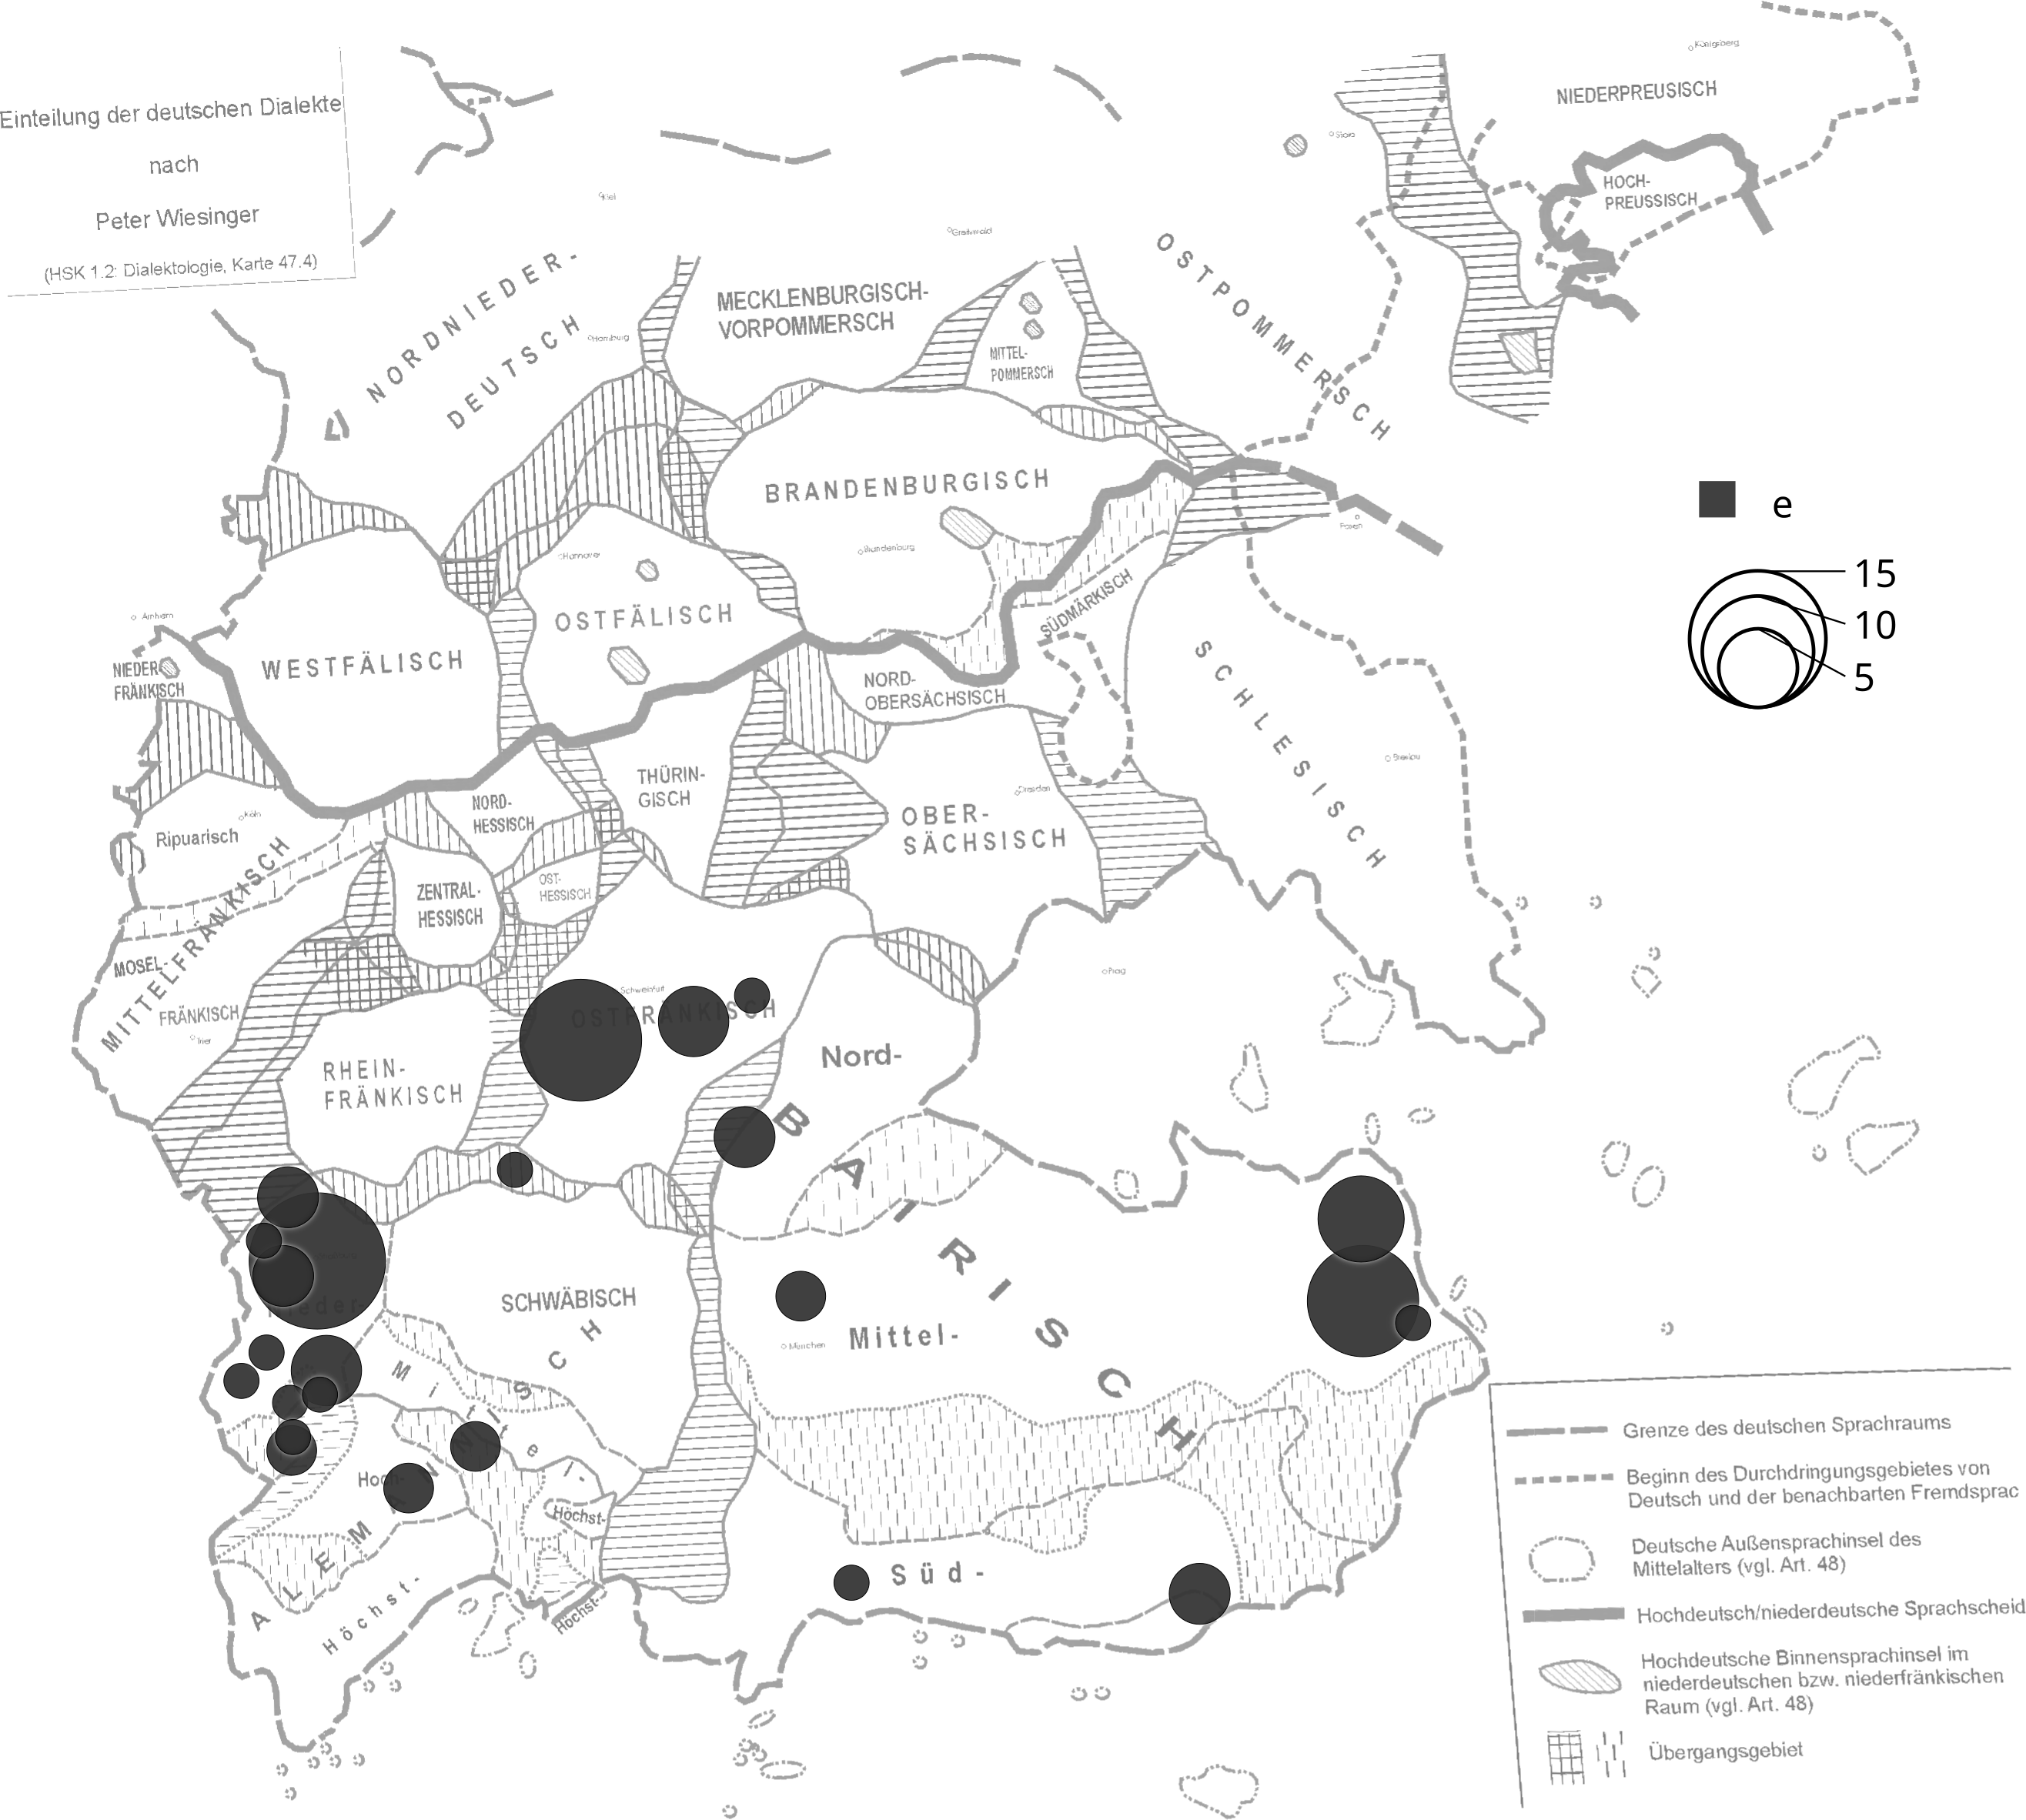
\includegraphics[
		height=.95\textheight,
		width=.49\linewidth,
		keepaspectratio
	]{./assets/grafiken/2021-10-11_cao_beide-conj.png}
}
~
\subfloat[\norm{bėidiu}]{
	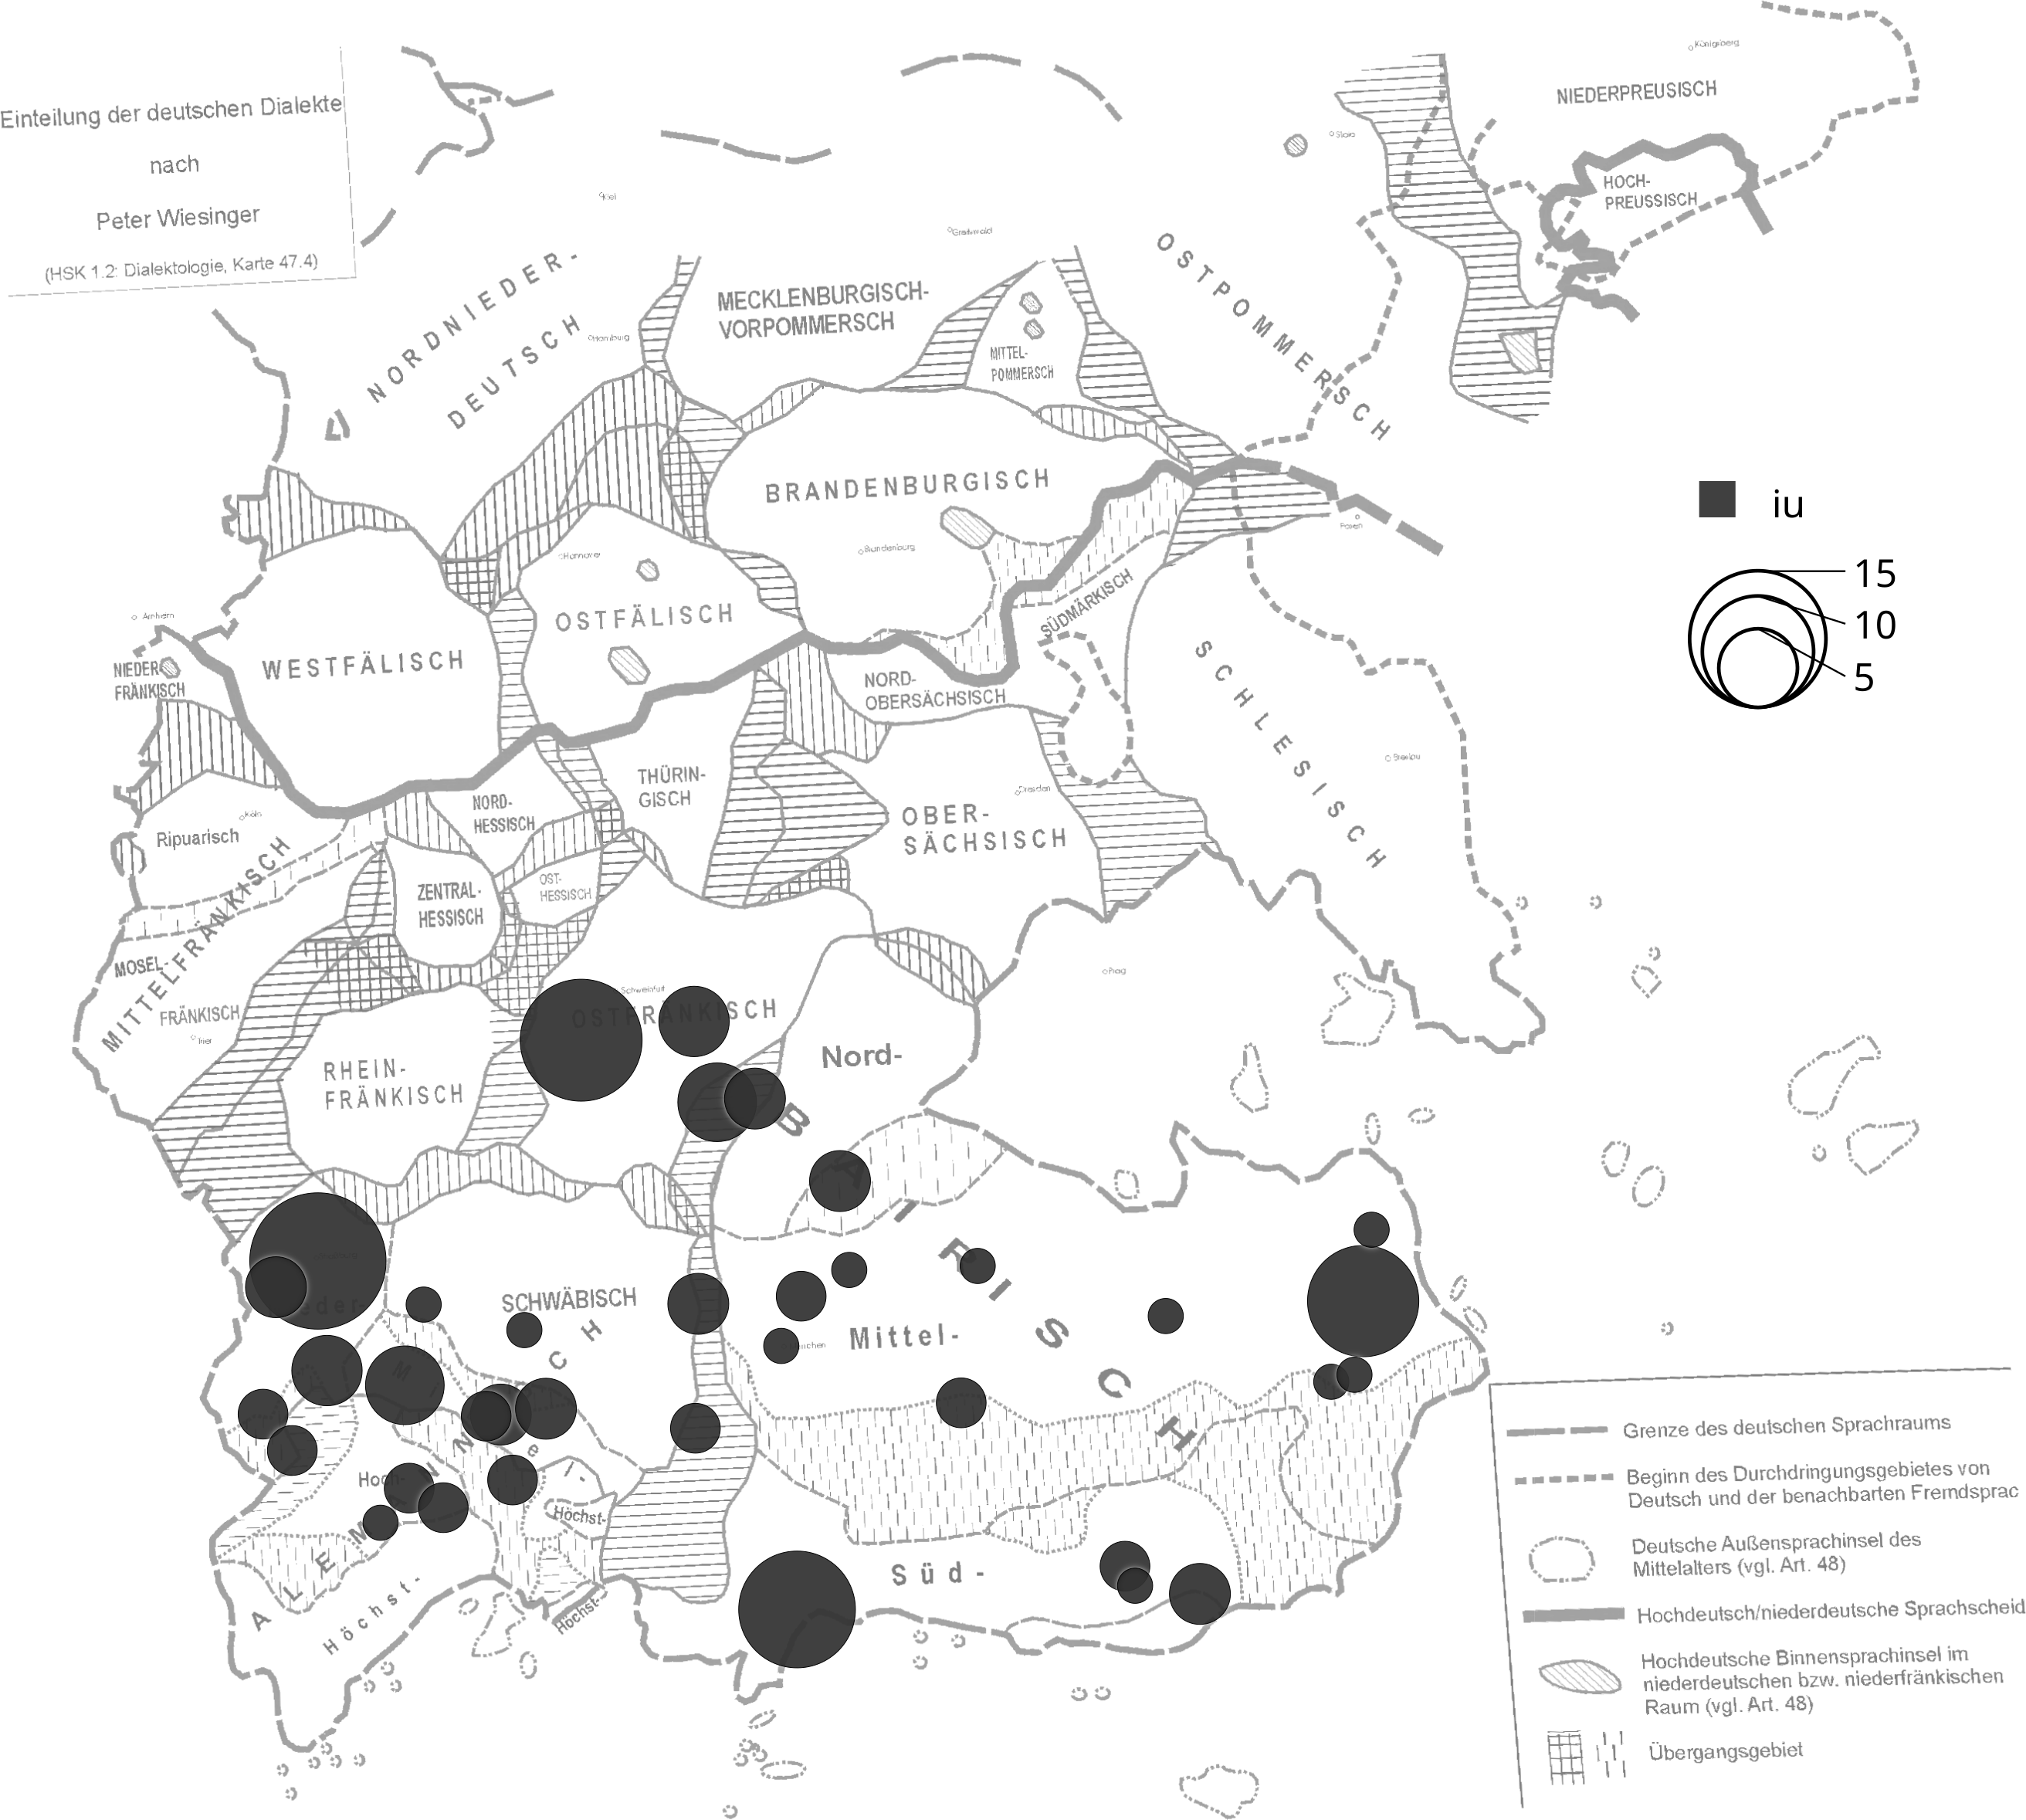
\includegraphics[
		height=.95\textheight,
		width=.49\linewidth,
		keepaspectratio
	]{./assets/grafiken/2021-10-11_cao_beidiu-conj.png}
}
\caption{Form der Konjunktion \norm{bėide \dots\ unde} \wdef{sowohl \dots\ als auch}}
\label{fig:cao_beideconj_geo}
\end{figure}
\end{landscape}
}

Wie bereits erwähnt, merkt \citet{gjelsten1980} an, dass es uneindeutige Fälle
von \norm{bėide \dots\ unde} gibt, die man \blockcquote[187]{gjelsten1980}{als
appositive Konstruktionen bewerten \textins{kann}, weil zwischen Pronomen und
kopulativer Fügung (Genus-)Kongruenz besteht, oder als konjunktionale
Konstruktionen, weil die Pronominalform als erstarrte konjunktionale
Konstituente interpretierbar ist}. Bei der Untersuchung haben sich im
exzerpierten Material aber keine Muster gezeigt, die eindeutig darauf
hindeuten, dass bei der Annotation der exzerpierten Belege regelmäßig
Apposition und Konjunktion verwechselt worden wären. Daneben liegen allerdings
die zwei Belege in \cref{ex:kczbeidenundesynt1} aus der \KC{}-Handschrift
\citet{kc:Z} vor, in denen \norm{bėide} eindeutig als Dativ flektiert
erscheint.

\begin{exe}
\ex \label{ex:kczbeidenundesynt1}
\begin{xlist}
	\ex \label{ex:kczbeidenundesynt1_1}
		\gll \textbf{Baiden} man vnd wib \\
			beide-\Dat.\Pl\subMF.\St{} Mann[\Dat.\Sg.\MascM] und
				Frau[\Dat.\Sg.\NeutF] \\
	\sn \gll Gebott er allen an den lyb \\
			gebot er all-\Dat.\Pl\subMF.\St{} an den Leib \\
		\begin{taggedline}{%
			\parencites[\pno~10\va, 9--10]{kc:Z}[vgl.]%
			[619--621]{schroeder1895}}
		\trans \wdef{Beiden, Mann und Frau, gebot er bei ihrem Leben}
		\end{taggedline}

\ex \label{ex:kczbeidenundesynt1_2}
	\gll \textbf{Baiden} man vnd wÿb \\
		beide-\Dat.\Pl\subMF.\St{} Mann[\Dat.\Sg.\MascM] und
			Frau[\Dat.\Sg.\NeutF] \\
\sn \gll Sol es gan an den lÿb \\
		soll es gehen an den Leib \\
	\begin{taggedline}{%
		\parencites[\pno~15\ra, 18--19]{kc:Z}%
		[zu][846--849]{schroeder1895}}
	\trans \wdef{Beiden, Mann und Frau, soll es ans Leben gehen.}
	\end{taggedline}
\end{xlist}
\end{exe}

Da im Plural eine Form vom Typ \norm{wīben} zu erwarten wäre, wurden die
Substantive hier als generisch verwendete Singulare aufgefasst. Das
kataphorische \lit{Baiden} bezieht sich zusammenfassend auf die nachfolgenden
Konjunkte. Da \norm{bėide} die Zweizahl in seiner Bedeutung definiert, ist
es notwendig, dass die beiden singularischen Konjunkte \norm{man} \wdef{Mann}
und \norm{wīp} ihre \Index-Merkmale zu einem Plural vereinigen, damit ein
zusammenhängender und wohlgeformter Ausdruck entsteht. Im Dat.~Pl.\ der starken
Adjektivdeklination spielt Genus keine Rolle, insofern kann diese Kategorie
hier vernachlässigt werden. Ansonsten wäre jedoch mit Gender Resolution zu
rechnen. Da Apposition vorliegt, muss \norm{bėide} genauso wie die Konjunkte im
Dativ stehen. \lit{Baiden} verkörpert also zusammen mit dem konkretisierenden
\norm{man unde wīp} das indirekte Objekt von \lit{gebott} \wdef{gebot}
beziehungsweise \lit{sol} \wdef{soll}.

Im Rahmen der LFG deuten \citet{sadlernordlinger2006} appositive Strukturen als
Variante von Koordination ohne overte Konjunktion. Sie diskutieren dies anhand
von Beispielen aus verschiedenen australischen Sprachen, in denen Koordination
von NPs durch einfache Nebeneinanderstellung der Konjunkte erreicht wird.
Darüber hinaus werde Nebeneinanderstellung aber nicht nur für asyndetische
Koordination von NPs verwendet, sondern auch für eine Reihe anderer,
\q*{Appositions-artiger} Konstruktionen
\autocite[440--441]{sadlernordlinger2006}. Für den vorliegenden Fall ist
lediglich wichtig, dass bei Koordination das \Index-Merkmal der Konjunkte
aufgelöst wird, bei Apposition hingegen nicht
\autocite[444]{sadlernordlinger2006}. Die Beispiele in
\cref{ex:kczbeidenundesynt1} lassen sich daher wie in
\cref{ex:kczbeidenundesynt2} dargestellt modellieren.

\begin{exe}
\ex \label{ex:kczbeidenundesynt2}
	\begin{forest}
		shorter edges,
		narrower nodes,
		italic leaves,
		align text,
	[{\anno[\pass{\SObj{recip}}]{DP\mysn{beidenunde_DP}}}
		[{\anno[\updownelem]{QP}}
			[\anno{\xhead{Q}}
				[{%
					bėiden, \\
					\smaller[2]\upshape\tabcolsep=.5ex%
					\begin{tabular}[t]{@{} l l l @{}}
						\ups{\GF~\Case} & \req & \Dat \\
						\ups{\GF~\Num} & \req & \Pl \\
					\end{tabular}%
				}]
			]
		]
		[{\anno[\updownelem]{NP}}
			[{\anno[\updownelem]{\xhead{N}}}
				[man]
			]
			[Conj
				[unde]
			]
			[{\anno[\updownelem]{\xhead{N}}}
				[wīp]
			]
		]
	]
	\end{forest}
	\quad
	\adjustbox{valign=t}{\smaller[2]%
		\avm{%
		\tikzmark{beidenunde_f}$f$: [
			\Conj	& \textit{appos} \\
			\mc{2}{l}{%
				\{
					$g_1$: [
						\Pred	& \wdef{beide}
					]~$i$, \smallskip \\

					$g_2$: [
						\Conj	& \textit{g-und} \\
						\mc{2}{l}{%
							\{
								$h_1$: [
									\Pred	& \wdef{Mann} \\
									\Pers	& \Third \\
									\Num	& \Sg \\
									\Gend	& \M \\
									\Sex	& \SM \\
									\Case	& \Dat
								], $h_2$: [
								 	\Pred	& \wdef{Frau} \\
								 	\Pers	& \Third \\
								 	\Num	& \Sg \\
								 	\Gend	& \N \\
								 	\Sex	& \SF \\
								 	\Case	& \Dat
								]
							\}%
						} \smallskip \\

						\Index	& [
							\Pers	& \Third \\
							\Gend	& \N \\
							\Num	& \Pl
						]
					]~$i$
				\}%
			}\smallskip \\
		\Index	& [
			\Pers	& \Third \\
			\Gend	& \N \\
			\Num	& \Pl
		] \\
	] \\
	}}
	\begin{tikzpicture}[remember picture, overlay]
	\draw [myarrow]
		([yshift=.5ex]{pic cs:beidenunde_DP})
		to [out=east, in=north west]
		([yshift=.5ex]{pic cs:beidenunde_f});
	\end{tikzpicture}
	\\
\end{exe}

In der F-Struktur auf der rechten Seite werden die Konjunkte \norm{man}
\wdef{Mann} und \norm{wīp} \wdef{Frau} in $g_2$ mit ihren grammatischen
Eigenschaften einzeln als $h_1$ und $h_2$ aufgelistet. Sie bilden zusammen
einen neuen \Index{} $i$, der die aufgelösten Personenmerkmale enthält. Sodann
bildet $g_1$ mit $g_2$ eine Apposition in $f$, wobei das Pronomen \norm{bėiden}
in $g_2$ mit $g_1$ koindiziert ist. Beide Teile zusammengenommen haben
ihrerseits ein \Index-Merkmal, das hier allerdings dem Index $i$ entspricht, da
$g_1$ keine neuen Informationen hinzufügt. In der C-Struktur auf der linken
Seite bilden \norm{man unde wīp} zusammen eine NP, die wiederum zusammen mit
der QP \norm{bėiden} eine DP bilden, die als indirektes Objekt dient.
